\documentclass[twoside]{book}

% Packages required by doxygen
\usepackage{fixltx2e}
\usepackage{calc}
\usepackage{doxygen}
\usepackage[export]{adjustbox} % also loads graphicx
\usepackage{graphicx}
\usepackage[utf8]{inputenc}
\usepackage{makeidx}
\usepackage{multicol}
\usepackage{multirow}
\PassOptionsToPackage{warn}{textcomp}
\usepackage{textcomp}
\usepackage[nointegrals]{wasysym}
\usepackage[table]{xcolor}

% Font selection
\usepackage[T1]{fontenc}
\usepackage[scaled=.90]{helvet}
\usepackage{courier}
\usepackage{amssymb}
\usepackage{sectsty}
\renewcommand{\familydefault}{\sfdefault}
\allsectionsfont{%
  \fontseries{bc}\selectfont%
  \color{darkgray}%
}
\renewcommand{\DoxyLabelFont}{%
  \fontseries{bc}\selectfont%
  \color{darkgray}%
}
\newcommand{\+}{\discretionary{\mbox{\scriptsize$\hookleftarrow$}}{}{}}

% Page & text layout
\usepackage{geometry}
\geometry{%
  a4paper,%
  top=2.5cm,%
  bottom=2.5cm,%
  left=2.5cm,%
  right=2.5cm%
}
\tolerance=750
\hfuzz=15pt
\hbadness=750
\setlength{\emergencystretch}{15pt}
\setlength{\parindent}{0cm}
\setlength{\parskip}{0.2cm}
\makeatletter
\renewcommand{\paragraph}{%
  \@startsection{paragraph}{4}{0ex}{-1.0ex}{1.0ex}{%
    \normalfont\normalsize\bfseries\SS@parafont%
  }%
}
\renewcommand{\subparagraph}{%
  \@startsection{subparagraph}{5}{0ex}{-1.0ex}{1.0ex}{%
    \normalfont\normalsize\bfseries\SS@subparafont%
  }%
}
\makeatother

% Headers & footers
\usepackage{fancyhdr}
\pagestyle{fancyplain}
\fancyhead[LE]{\fancyplain{}{\bfseries\thepage}}
\fancyhead[CE]{\fancyplain{}{}}
\fancyhead[RE]{\fancyplain{}{\bfseries\leftmark}}
\fancyhead[LO]{\fancyplain{}{\bfseries\rightmark}}
\fancyhead[CO]{\fancyplain{}{}}
\fancyhead[RO]{\fancyplain{}{\bfseries\thepage}}
\fancyfoot[LE]{\fancyplain{}{}}
\fancyfoot[CE]{\fancyplain{}{}}
\fancyfoot[RE]{\fancyplain{}{\bfseries\scriptsize Generated on Sat Jul 4 2015 17\+:36\+:10 for Pyccuweather by Doxygen }}
\fancyfoot[LO]{\fancyplain{}{\bfseries\scriptsize Generated on Sat Jul 4 2015 17\+:36\+:10 for Pyccuweather by Doxygen }}
\fancyfoot[CO]{\fancyplain{}{}}
\fancyfoot[RO]{\fancyplain{}{}}
\renewcommand{\footrulewidth}{0.4pt}
\renewcommand{\chaptermark}[1]{%
  \markboth{#1}{}%
}
\renewcommand{\sectionmark}[1]{%
  \markright{\thesection\ #1}%
}

% Indices & bibliography
\usepackage{natbib}
\usepackage[titles]{tocloft}
\setcounter{tocdepth}{3}
\setcounter{secnumdepth}{5}
\makeindex

% Hyperlinks (required, but should be loaded last)
\usepackage{ifpdf}
\ifpdf
  \usepackage[pdftex,pagebackref=true]{hyperref}
\else
  \usepackage[ps2pdf,pagebackref=true]{hyperref}
\fi
\hypersetup{%
  colorlinks=true,%
  linkcolor=blue,%
  citecolor=blue,%
  unicode%
}

% Custom commands
\newcommand{\clearemptydoublepage}{%
  \newpage{\pagestyle{empty}\cleardoublepage}%
}


%===== C O N T E N T S =====

\begin{document}

% Titlepage & ToC
\hypersetup{pageanchor=false,
             bookmarks=true,
             bookmarksnumbered=true,
             pdfencoding=unicode
            }
\pagenumbering{roman}
\begin{titlepage}
\vspace*{7cm}
\begin{center}%
{\Large Pyccuweather \\[1ex]\large 0.\+31 }\\
\vspace*{1cm}
{\large Generated by Doxygen 1.8.9.1}\\
\vspace*{0.5cm}
{\small Sat Jul 4 2015 17:36:10}\\
\end{center}
\end{titlepage}
\clearemptydoublepage
\tableofcontents
\clearemptydoublepage
\pagenumbering{arabic}
\hypersetup{pageanchor=true}

%--- Begin generated contents ---
\chapter{Hierarchical Index}
\section{Class Hierarchy}
This inheritance list is sorted roughly, but not completely, alphabetically\+:\begin{DoxyCompactList}
\item Base\+Exception\begin{DoxyCompactList}
\item \contentsline{section}{pyccuweather.\+errors.\+A\+P\+I\+Connection\+Error}{\pageref{classpyccuweather_1_1errors_1_1_a_p_i_connection_error}}{}
\item \contentsline{section}{pyccuweather.\+errors.\+A\+P\+I\+Error}{\pageref{classpyccuweather_1_1errors_1_1_a_p_i_error}}{}
\item \contentsline{section}{pyccuweather.\+errors.\+Invalid\+Country\+Code\+Error}{\pageref{classpyccuweather_1_1errors_1_1_invalid_country_code_error}}{}
\item \contentsline{section}{pyccuweather.\+errors.\+Malformatted\+A\+P\+I\+Key\+Error}{\pageref{classpyccuweather_1_1errors_1_1_malformatted_a_p_i_key_error}}{}
\item \contentsline{section}{pyccuweather.\+errors.\+Malformatted\+Location\+Key\+Error}{\pageref{classpyccuweather_1_1errors_1_1_malformatted_location_key_error}}{}
\item \contentsline{section}{pyccuweather.\+errors.\+No\+Location\+Error}{\pageref{classpyccuweather_1_1errors_1_1_no_location_error}}{}
\item \contentsline{section}{pyccuweather.\+errors.\+No\+Results\+Error}{\pageref{classpyccuweather_1_1errors_1_1_no_results_error}}{}
\item \contentsline{section}{pyccuweather.\+errors.\+Not\+Implemented\+Or\+Unknown\+Method}{\pageref{classpyccuweather_1_1errors_1_1_not_implemented_or_unknown_method}}{}
\item \contentsline{section}{pyccuweather.\+errors.\+Range\+Error}{\pageref{classpyccuweather_1_1errors_1_1_range_error}}{}
\item \contentsline{section}{pyccuweather.\+errors.\+Unauthorised\+Error}{\pageref{classpyccuweather_1_1errors_1_1_unauthorised_error}}{}
\end{DoxyCompactList}
\item object\begin{DoxyCompactList}
\item \contentsline{section}{pyccuweather.\+connector.\+Connection}{\pageref{classpyccuweather_1_1connector_1_1_connection}}{}
\item \contentsline{section}{pyccuweather.\+objects.\+Administrative\+Area}{\pageref{classpyccuweather_1_1objects_1_1_administrative_area}}{}
\item \contentsline{section}{pyccuweather.\+objects.\+Air\+Quality}{\pageref{classpyccuweather_1_1objects_1_1_air_quality}}{}
\item \contentsline{section}{pyccuweather.\+objects.\+Air\+Quality\+Factor}{\pageref{classpyccuweather_1_1objects_1_1_air_quality_factor}}{}
\item \contentsline{section}{pyccuweather.\+objects.\+Ceiling}{\pageref{classpyccuweather_1_1objects_1_1_ceiling}}{}
\item \contentsline{section}{pyccuweather.\+objects.\+Country}{\pageref{classpyccuweather_1_1objects_1_1_country}}{}
\item \contentsline{section}{pyccuweather.\+objects.\+Current\+Obs}{\pageref{classpyccuweather_1_1objects_1_1_current_obs}}{}
\item \contentsline{section}{pyccuweather.\+objects.\+Daily\+Forecast}{\pageref{classpyccuweather_1_1objects_1_1_daily_forecast}}{}
\item \contentsline{section}{pyccuweather.\+objects.\+Daily\+Forecasts}{\pageref{classpyccuweather_1_1objects_1_1_daily_forecasts}}{}
\item \contentsline{section}{pyccuweather.\+objects.\+Degree\+Day}{\pageref{classpyccuweather_1_1objects_1_1_degree_day}}{}
\item \contentsline{section}{pyccuweather.\+objects.\+Hemiurnal}{\pageref{classpyccuweather_1_1objects_1_1_hemiurnal}}{}
\item \contentsline{section}{pyccuweather.\+objects.\+Hourly\+Forecast}{\pageref{classpyccuweather_1_1objects_1_1_hourly_forecast}}{}
\item \contentsline{section}{pyccuweather.\+objects.\+Hourly\+Forecasts}{\pageref{classpyccuweather_1_1objects_1_1_hourly_forecasts}}{}
\item \contentsline{section}{pyccuweather.\+objects.\+Location}{\pageref{classpyccuweather_1_1objects_1_1_location}}{}
\item \contentsline{section}{pyccuweather.\+objects.\+Location\+Set}{\pageref{classpyccuweather_1_1objects_1_1_location_set}}{}
\item \contentsline{section}{pyccuweather.\+objects.\+Observation}{\pageref{classpyccuweather_1_1objects_1_1_observation}}{}
\item \contentsline{section}{pyccuweather.\+objects.\+Precipitation}{\pageref{classpyccuweather_1_1objects_1_1_precipitation}}{}
\item \contentsline{section}{pyccuweather.\+objects.\+Region}{\pageref{classpyccuweather_1_1objects_1_1_region}}{}
\item \contentsline{section}{pyccuweather.\+objects.\+Snow}{\pageref{classpyccuweather_1_1objects_1_1_snow}}{}
\item \contentsline{section}{pyccuweather.\+objects.\+Temperature}{\pageref{classpyccuweather_1_1objects_1_1_temperature}}{}
\item \contentsline{section}{pyccuweather.\+objects.\+Time\+Zone}{\pageref{classpyccuweather_1_1objects_1_1_time_zone}}{}
\item \contentsline{section}{pyccuweather.\+objects.\+Wind}{\pageref{classpyccuweather_1_1objects_1_1_wind}}{}
\end{DoxyCompactList}
\end{DoxyCompactList}

\chapter{Class Index}
\section{Class List}
Here are the classes, structs, unions and interfaces with brief descriptions\+:\begin{DoxyCompactList}
\item\contentsline{section}{\hyperlink{classpyccuweather_1_1objects_1_1_administrative_area}{pyccuweather.\+objects.\+Administrative\+Area} }{\pageref{classpyccuweather_1_1objects_1_1_administrative_area}}{}
\item\contentsline{section}{\hyperlink{classpyccuweather_1_1objects_1_1_air_quality}{pyccuweather.\+objects.\+Air\+Quality} }{\pageref{classpyccuweather_1_1objects_1_1_air_quality}}{}
\item\contentsline{section}{\hyperlink{classpyccuweather_1_1objects_1_1_air_quality_factor}{pyccuweather.\+objects.\+Air\+Quality\+Factor} }{\pageref{classpyccuweather_1_1objects_1_1_air_quality_factor}}{}
\item\contentsline{section}{\hyperlink{classpyccuweather_1_1errors_1_1_a_p_i_connection_error}{pyccuweather.\+errors.\+A\+P\+I\+Connection\+Error} }{\pageref{classpyccuweather_1_1errors_1_1_a_p_i_connection_error}}{}
\item\contentsline{section}{\hyperlink{classpyccuweather_1_1errors_1_1_a_p_i_error}{pyccuweather.\+errors.\+A\+P\+I\+Error} }{\pageref{classpyccuweather_1_1errors_1_1_a_p_i_error}}{}
\item\contentsline{section}{\hyperlink{classpyccuweather_1_1objects_1_1_ceiling}{pyccuweather.\+objects.\+Ceiling} }{\pageref{classpyccuweather_1_1objects_1_1_ceiling}}{}
\item\contentsline{section}{\hyperlink{classpyccuweather_1_1connector_1_1_connection}{pyccuweather.\+connector.\+Connection} }{\pageref{classpyccuweather_1_1connector_1_1_connection}}{}
\item\contentsline{section}{\hyperlink{classpyccuweather_1_1objects_1_1_country}{pyccuweather.\+objects.\+Country} }{\pageref{classpyccuweather_1_1objects_1_1_country}}{}
\item\contentsline{section}{\hyperlink{classpyccuweather_1_1objects_1_1_current_obs}{pyccuweather.\+objects.\+Current\+Obs} }{\pageref{classpyccuweather_1_1objects_1_1_current_obs}}{}
\item\contentsline{section}{\hyperlink{classpyccuweather_1_1objects_1_1_daily_forecast}{pyccuweather.\+objects.\+Daily\+Forecast} }{\pageref{classpyccuweather_1_1objects_1_1_daily_forecast}}{}
\item\contentsline{section}{\hyperlink{classpyccuweather_1_1objects_1_1_daily_forecasts}{pyccuweather.\+objects.\+Daily\+Forecasts} }{\pageref{classpyccuweather_1_1objects_1_1_daily_forecasts}}{}
\item\contentsline{section}{\hyperlink{classpyccuweather_1_1objects_1_1_degree_day}{pyccuweather.\+objects.\+Degree\+Day} }{\pageref{classpyccuweather_1_1objects_1_1_degree_day}}{}
\item\contentsline{section}{\hyperlink{classpyccuweather_1_1objects_1_1_hemiurnal}{pyccuweather.\+objects.\+Hemiurnal} }{\pageref{classpyccuweather_1_1objects_1_1_hemiurnal}}{}
\item\contentsline{section}{\hyperlink{classpyccuweather_1_1objects_1_1_hourly_forecast}{pyccuweather.\+objects.\+Hourly\+Forecast} }{\pageref{classpyccuweather_1_1objects_1_1_hourly_forecast}}{}
\item\contentsline{section}{\hyperlink{classpyccuweather_1_1objects_1_1_hourly_forecasts}{pyccuweather.\+objects.\+Hourly\+Forecasts} }{\pageref{classpyccuweather_1_1objects_1_1_hourly_forecasts}}{}
\item\contentsline{section}{\hyperlink{classpyccuweather_1_1errors_1_1_invalid_country_code_error}{pyccuweather.\+errors.\+Invalid\+Country\+Code\+Error} }{\pageref{classpyccuweather_1_1errors_1_1_invalid_country_code_error}}{}
\item\contentsline{section}{\hyperlink{classpyccuweather_1_1objects_1_1_location}{pyccuweather.\+objects.\+Location} }{\pageref{classpyccuweather_1_1objects_1_1_location}}{}
\item\contentsline{section}{\hyperlink{classpyccuweather_1_1objects_1_1_location_set}{pyccuweather.\+objects.\+Location\+Set} }{\pageref{classpyccuweather_1_1objects_1_1_location_set}}{}
\item\contentsline{section}{\hyperlink{classpyccuweather_1_1errors_1_1_malformatted_a_p_i_key_error}{pyccuweather.\+errors.\+Malformatted\+A\+P\+I\+Key\+Error} }{\pageref{classpyccuweather_1_1errors_1_1_malformatted_a_p_i_key_error}}{}
\item\contentsline{section}{\hyperlink{classpyccuweather_1_1errors_1_1_malformatted_location_key_error}{pyccuweather.\+errors.\+Malformatted\+Location\+Key\+Error} }{\pageref{classpyccuweather_1_1errors_1_1_malformatted_location_key_error}}{}
\item\contentsline{section}{\hyperlink{classpyccuweather_1_1errors_1_1_no_location_error}{pyccuweather.\+errors.\+No\+Location\+Error} }{\pageref{classpyccuweather_1_1errors_1_1_no_location_error}}{}
\item\contentsline{section}{\hyperlink{classpyccuweather_1_1errors_1_1_no_results_error}{pyccuweather.\+errors.\+No\+Results\+Error} }{\pageref{classpyccuweather_1_1errors_1_1_no_results_error}}{}
\item\contentsline{section}{\hyperlink{classpyccuweather_1_1errors_1_1_not_implemented_or_unknown_method}{pyccuweather.\+errors.\+Not\+Implemented\+Or\+Unknown\+Method} }{\pageref{classpyccuweather_1_1errors_1_1_not_implemented_or_unknown_method}}{}
\item\contentsline{section}{\hyperlink{classpyccuweather_1_1objects_1_1_observation}{pyccuweather.\+objects.\+Observation} }{\pageref{classpyccuweather_1_1objects_1_1_observation}}{}
\item\contentsline{section}{\hyperlink{classpyccuweather_1_1objects_1_1_precipitation}{pyccuweather.\+objects.\+Precipitation} }{\pageref{classpyccuweather_1_1objects_1_1_precipitation}}{}
\item\contentsline{section}{\hyperlink{classpyccuweather_1_1errors_1_1_range_error}{pyccuweather.\+errors.\+Range\+Error} }{\pageref{classpyccuweather_1_1errors_1_1_range_error}}{}
\item\contentsline{section}{\hyperlink{classpyccuweather_1_1objects_1_1_region}{pyccuweather.\+objects.\+Region} }{\pageref{classpyccuweather_1_1objects_1_1_region}}{}
\item\contentsline{section}{\hyperlink{classpyccuweather_1_1objects_1_1_snow}{pyccuweather.\+objects.\+Snow} }{\pageref{classpyccuweather_1_1objects_1_1_snow}}{}
\item\contentsline{section}{\hyperlink{classpyccuweather_1_1objects_1_1_temperature}{pyccuweather.\+objects.\+Temperature} }{\pageref{classpyccuweather_1_1objects_1_1_temperature}}{}
\item\contentsline{section}{\hyperlink{classpyccuweather_1_1objects_1_1_time_zone}{pyccuweather.\+objects.\+Time\+Zone} }{\pageref{classpyccuweather_1_1objects_1_1_time_zone}}{}
\item\contentsline{section}{\hyperlink{classpyccuweather_1_1errors_1_1_unauthorised_error}{pyccuweather.\+errors.\+Unauthorised\+Error} }{\pageref{classpyccuweather_1_1errors_1_1_unauthorised_error}}{}
\item\contentsline{section}{\hyperlink{classpyccuweather_1_1objects_1_1_wind}{pyccuweather.\+objects.\+Wind} }{\pageref{classpyccuweather_1_1objects_1_1_wind}}{}
\end{DoxyCompactList}

\chapter{Class Documentation}
\hypertarget{classpyccuweather_1_1objects_1_1_administrative_area}{}\section{pyccuweather.\+objects.\+Administrative\+Area Class Reference}
\label{classpyccuweather_1_1objects_1_1_administrative_area}\index{pyccuweather.\+objects.\+Administrative\+Area@{pyccuweather.\+objects.\+Administrative\+Area}}
Inheritance diagram for pyccuweather.\+objects.\+Administrative\+Area\+:\begin{figure}[H]
\begin{center}
\leavevmode
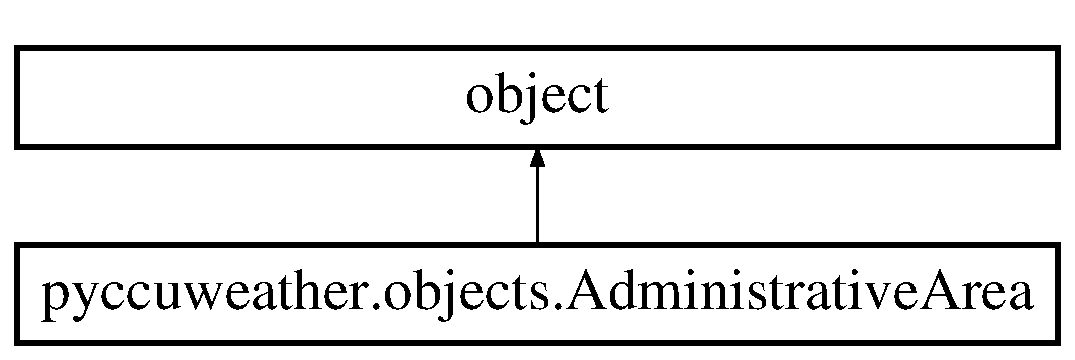
\includegraphics[height=2.000000cm]{classpyccuweather_1_1objects_1_1_administrative_area}
\end{center}
\end{figure}
\subsection*{Public Member Functions}
\begin{DoxyCompactItemize}
\item 
\hypertarget{classpyccuweather_1_1objects_1_1_administrative_area_a40ce4cc3d820f593039493c821a9b959}{}def {\bfseries \+\_\+\+\_\+init\+\_\+\+\_\+}\label{classpyccuweather_1_1objects_1_1_administrative_area_a40ce4cc3d820f593039493c821a9b959}

\item 
\hypertarget{classpyccuweather_1_1objects_1_1_administrative_area_ab0451305c0002cc06e8ebab5c04d75fe}{}def {\bfseries \+\_\+\+\_\+str\+\_\+\+\_\+} (self)\label{classpyccuweather_1_1objects_1_1_administrative_area_ab0451305c0002cc06e8ebab5c04d75fe}

\end{DoxyCompactItemize}
\subsection*{Public Attributes}
\begin{DoxyCompactItemize}
\item 
\hypertarget{classpyccuweather_1_1objects_1_1_administrative_area_aac1366c9c319b1f5bd29f1462d11908a}{}{\bfseries id}\label{classpyccuweather_1_1objects_1_1_administrative_area_aac1366c9c319b1f5bd29f1462d11908a}

\item 
\hypertarget{classpyccuweather_1_1objects_1_1_administrative_area_ae6387b8697e0c131244f2723c182a9a4}{}{\bfseries localized\+\_\+name}\label{classpyccuweather_1_1objects_1_1_administrative_area_ae6387b8697e0c131244f2723c182a9a4}

\item 
\hypertarget{classpyccuweather_1_1objects_1_1_administrative_area_ac68e966ae1fef389f04ed777fb6dbfed}{}{\bfseries english\+\_\+name}\label{classpyccuweather_1_1objects_1_1_administrative_area_ac68e966ae1fef389f04ed777fb6dbfed}

\item 
\hypertarget{classpyccuweather_1_1objects_1_1_administrative_area_a0d8c5202b19824d2c280868c22c027c0}{}{\bfseries level}\label{classpyccuweather_1_1objects_1_1_administrative_area_a0d8c5202b19824d2c280868c22c027c0}

\item 
\hypertarget{classpyccuweather_1_1objects_1_1_administrative_area_a3e92d8a22d8cc63a105933cc4fa3cbc2}{}{\bfseries localized\+\_\+type}\label{classpyccuweather_1_1objects_1_1_administrative_area_a3e92d8a22d8cc63a105933cc4fa3cbc2}

\item 
\hypertarget{classpyccuweather_1_1objects_1_1_administrative_area_a3d6b44091e48f19da021c2d9564d2c29}{}{\bfseries english\+\_\+type}\label{classpyccuweather_1_1objects_1_1_administrative_area_a3d6b44091e48f19da021c2d9564d2c29}

\end{DoxyCompactItemize}


\subsection{Detailed Description}
\begin{DoxyVerb}Represents a primary administrative area.
Countries are explained in the Accuweather documentation at http://apidev.accuweather.com/developers/administrativeareas
\end{DoxyVerb}
 

The documentation for this class was generated from the following file\+:\begin{DoxyCompactItemize}
\item 
pyccuweather/objects.\+py\end{DoxyCompactItemize}

\hypertarget{classpyccuweather_1_1objects_1_1_air_quality}{}\section{pyccuweather.\+objects.\+Air\+Quality Class Reference}
\label{classpyccuweather_1_1objects_1_1_air_quality}\index{pyccuweather.\+objects.\+Air\+Quality@{pyccuweather.\+objects.\+Air\+Quality}}
Inheritance diagram for pyccuweather.\+objects.\+Air\+Quality\+:\begin{figure}[H]
\begin{center}
\leavevmode
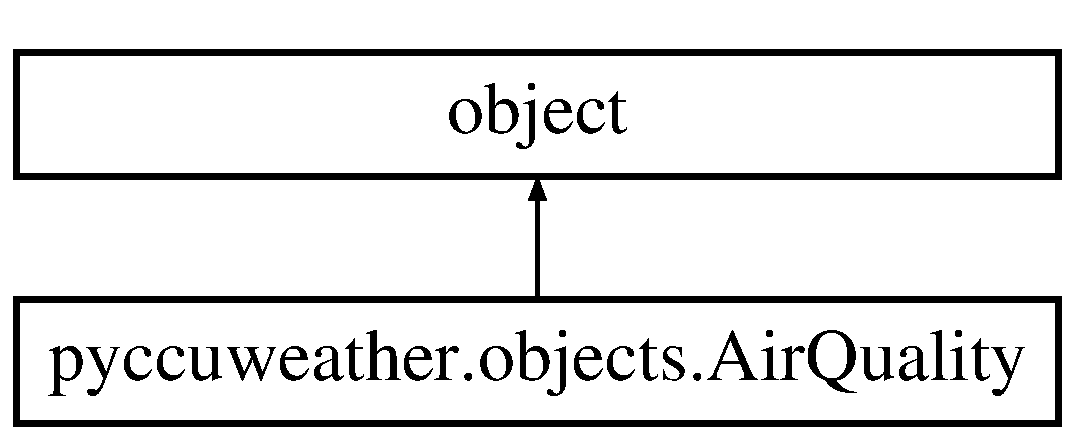
\includegraphics[height=2.000000cm]{classpyccuweather_1_1objects_1_1_air_quality}
\end{center}
\end{figure}
\subsection*{Public Member Functions}
\begin{DoxyCompactItemize}
\item 
\hypertarget{classpyccuweather_1_1objects_1_1_air_quality_aa7e6eba5756b729f13b89532a00cff31}{}def {\bfseries \+\_\+\+\_\+init\+\_\+\+\_\+} (self, aqf\+\_\+dict)\label{classpyccuweather_1_1objects_1_1_air_quality_aa7e6eba5756b729f13b89532a00cff31}

\end{DoxyCompactItemize}


The documentation for this class was generated from the following file\+:\begin{DoxyCompactItemize}
\item 
pyccuweather/objects.\+py\end{DoxyCompactItemize}

\hypertarget{classpyccuweather_1_1objects_1_1_air_quality_factor}{}\section{pyccuweather.\+objects.\+Air\+Quality\+Factor Class Reference}
\label{classpyccuweather_1_1objects_1_1_air_quality_factor}\index{pyccuweather.\+objects.\+Air\+Quality\+Factor@{pyccuweather.\+objects.\+Air\+Quality\+Factor}}
Inheritance diagram for pyccuweather.\+objects.\+Air\+Quality\+Factor\+:\begin{figure}[H]
\begin{center}
\leavevmode
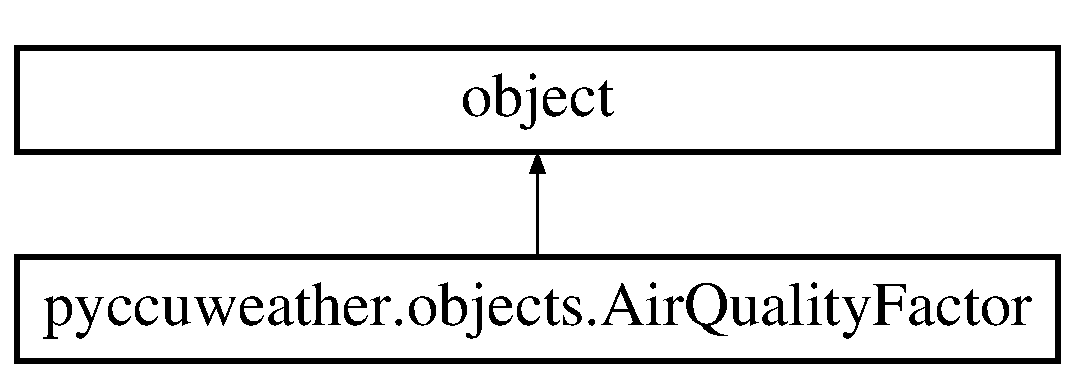
\includegraphics[height=2.000000cm]{classpyccuweather_1_1objects_1_1_air_quality_factor}
\end{center}
\end{figure}
\subsection*{Public Member Functions}
\begin{DoxyCompactItemize}
\item 
\hypertarget{classpyccuweather_1_1objects_1_1_air_quality_factor_a4834573080320fa3126146e47dc019e2}{}def {\bfseries \+\_\+\+\_\+init\+\_\+\+\_\+} (self, aqf\+\_\+dict)\label{classpyccuweather_1_1objects_1_1_air_quality_factor_a4834573080320fa3126146e47dc019e2}

\item 
\hypertarget{classpyccuweather_1_1objects_1_1_air_quality_factor_aac494b7df4807a2f87aa09e2f516dc7b}{}def {\bfseries \+\_\+\+\_\+str\+\_\+\+\_\+} (self)\label{classpyccuweather_1_1objects_1_1_air_quality_factor_aac494b7df4807a2f87aa09e2f516dc7b}

\end{DoxyCompactItemize}
\subsection*{Public Attributes}
\begin{DoxyCompactItemize}
\item 
\hypertarget{classpyccuweather_1_1objects_1_1_air_quality_factor_ad388f6fa1500cbe907e8ba5617ac57da}{}{\bfseries name}\label{classpyccuweather_1_1objects_1_1_air_quality_factor_ad388f6fa1500cbe907e8ba5617ac57da}

\item 
\hypertarget{classpyccuweather_1_1objects_1_1_air_quality_factor_a08a597e10fff0646c8c39b2aa24bb43b}{}{\bfseries value}\label{classpyccuweather_1_1objects_1_1_air_quality_factor_a08a597e10fff0646c8c39b2aa24bb43b}

\item 
\hypertarget{classpyccuweather_1_1objects_1_1_air_quality_factor_a0f77a25c68fd5038a2ffa5b299a59bf4}{}{\bfseries category}\label{classpyccuweather_1_1objects_1_1_air_quality_factor_a0f77a25c68fd5038a2ffa5b299a59bf4}

\item 
\hypertarget{classpyccuweather_1_1objects_1_1_air_quality_factor_a50ed11d0ea62a26199cc75fa55760525}{}{\bfseries band}\label{classpyccuweather_1_1objects_1_1_air_quality_factor_a50ed11d0ea62a26199cc75fa55760525}

\end{DoxyCompactItemize}


The documentation for this class was generated from the following file\+:\begin{DoxyCompactItemize}
\item 
pyccuweather/objects.\+py\end{DoxyCompactItemize}

\hypertarget{classpyccuweather_1_1errors_1_1_a_p_i_connection_error}{}\section{pyccuweather.\+errors.\+A\+P\+I\+Connection\+Error Class Reference}
\label{classpyccuweather_1_1errors_1_1_a_p_i_connection_error}\index{pyccuweather.\+errors.\+A\+P\+I\+Connection\+Error@{pyccuweather.\+errors.\+A\+P\+I\+Connection\+Error}}
Inheritance diagram for pyccuweather.\+errors.\+A\+P\+I\+Connection\+Error\+:\begin{figure}[H]
\begin{center}
\leavevmode
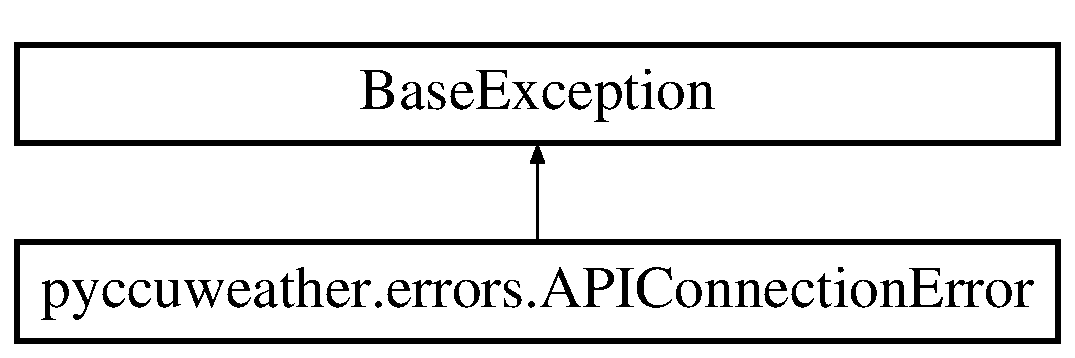
\includegraphics[height=2.000000cm]{classpyccuweather_1_1errors_1_1_a_p_i_connection_error}
\end{center}
\end{figure}
\subsection*{Public Member Functions}
\begin{DoxyCompactItemize}
\item 
\hypertarget{classpyccuweather_1_1errors_1_1_a_p_i_connection_error_a515e0937a6f37a9b3d5f76477d1feb09}{}def {\bfseries \+\_\+\+\_\+str\+\_\+\+\_\+} (self)\label{classpyccuweather_1_1errors_1_1_a_p_i_connection_error_a515e0937a6f37a9b3d5f76477d1feb09}

\end{DoxyCompactItemize}


\subsection{Detailed Description}
\begin{DoxyVerb}Raised when no connection to the Accuweather servers could be established.
\end{DoxyVerb}
 

The documentation for this class was generated from the following file\+:\begin{DoxyCompactItemize}
\item 
pyccuweather/errors.\+py\end{DoxyCompactItemize}

\hypertarget{classpyccuweather_1_1errors_1_1_a_p_i_error}{}\section{pyccuweather.\+errors.\+A\+P\+I\+Error Class Reference}
\label{classpyccuweather_1_1errors_1_1_a_p_i_error}\index{pyccuweather.\+errors.\+A\+P\+I\+Error@{pyccuweather.\+errors.\+A\+P\+I\+Error}}
Inheritance diagram for pyccuweather.\+errors.\+A\+P\+I\+Error\+:\begin{figure}[H]
\begin{center}
\leavevmode
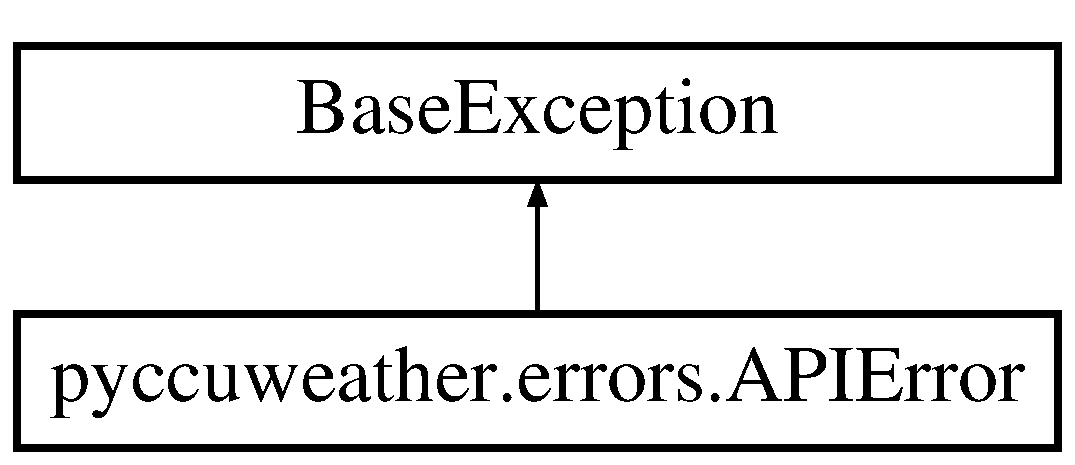
\includegraphics[height=2.000000cm]{classpyccuweather_1_1errors_1_1_a_p_i_error}
\end{center}
\end{figure}
\subsection*{Public Member Functions}
\begin{DoxyCompactItemize}
\item 
\hypertarget{classpyccuweather_1_1errors_1_1_a_p_i_error_a8d29dd91479ec96b56213b0c38232869}{}def {\bfseries \+\_\+\+\_\+init\+\_\+\+\_\+} (self, status\+\_\+code)\label{classpyccuweather_1_1errors_1_1_a_p_i_error_a8d29dd91479ec96b56213b0c38232869}

\item 
\hypertarget{classpyccuweather_1_1errors_1_1_a_p_i_error_a0fedcce781a53c3e8914370aa62bcf41}{}def {\bfseries \+\_\+\+\_\+str\+\_\+\+\_\+} (self)\label{classpyccuweather_1_1errors_1_1_a_p_i_error_a0fedcce781a53c3e8914370aa62bcf41}

\end{DoxyCompactItemize}
\subsection*{Public Attributes}
\begin{DoxyCompactItemize}
\item 
\hypertarget{classpyccuweather_1_1errors_1_1_a_p_i_error_aacf9ec6422944075b248b3b3c53af924}{}{\bfseries status\+\_\+code}\label{classpyccuweather_1_1errors_1_1_a_p_i_error_aacf9ec6422944075b248b3b3c53af924}

\end{DoxyCompactItemize}


\subsection{Detailed Description}
\begin{DoxyVerb}Raised when the Accuweather servers returned a HTTP error code.
\end{DoxyVerb}
 

The documentation for this class was generated from the following file\+:\begin{DoxyCompactItemize}
\item 
pyccuweather/errors.\+py\end{DoxyCompactItemize}

\hypertarget{classpyccuweather_1_1objects_1_1_ceiling}{}\section{pyccuweather.\+objects.\+Ceiling Class Reference}
\label{classpyccuweather_1_1objects_1_1_ceiling}\index{pyccuweather.\+objects.\+Ceiling@{pyccuweather.\+objects.\+Ceiling}}
Inheritance diagram for pyccuweather.\+objects.\+Ceiling\+:\begin{figure}[H]
\begin{center}
\leavevmode
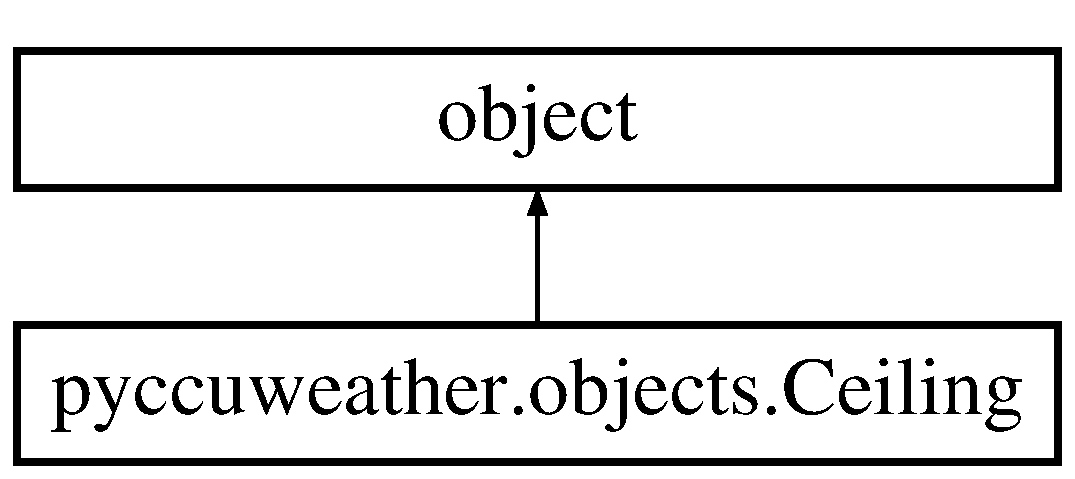
\includegraphics[height=2.000000cm]{classpyccuweather_1_1objects_1_1_ceiling}
\end{center}
\end{figure}
\subsection*{Public Member Functions}
\begin{DoxyCompactItemize}
\item 
\hypertarget{classpyccuweather_1_1objects_1_1_ceiling_af7fe23b0aaf54a2fb65c3eb84ad4e1c7}{}def {\bfseries \+\_\+\+\_\+init\+\_\+\+\_\+} (self, json)\label{classpyccuweather_1_1objects_1_1_ceiling_af7fe23b0aaf54a2fb65c3eb84ad4e1c7}

\item 
\hypertarget{classpyccuweather_1_1objects_1_1_ceiling_a1d008acce4cfa083a630f90d2f7df1ed}{}def {\bfseries km} (self)\label{classpyccuweather_1_1objects_1_1_ceiling_a1d008acce4cfa083a630f90d2f7df1ed}

\item 
\hypertarget{classpyccuweather_1_1objects_1_1_ceiling_a3e0573256e81df1d015bfb639ec8f914}{}def {\bfseries m} (self)\label{classpyccuweather_1_1objects_1_1_ceiling_a3e0573256e81df1d015bfb639ec8f914}

\item 
\hypertarget{classpyccuweather_1_1objects_1_1_ceiling_a3c43f091db846ee0bac342cb48184e66}{}def {\bfseries ft} (self)\label{classpyccuweather_1_1objects_1_1_ceiling_a3c43f091db846ee0bac342cb48184e66}

\item 
\hypertarget{classpyccuweather_1_1objects_1_1_ceiling_a6a0b00a2bb4679c88a4cc6388832cdc1}{}def {\bfseries \+\_\+\+\_\+str\+\_\+\+\_\+} (self)\label{classpyccuweather_1_1objects_1_1_ceiling_a6a0b00a2bb4679c88a4cc6388832cdc1}

\end{DoxyCompactItemize}
\subsection*{Public Attributes}
\begin{DoxyCompactItemize}
\item 
\hypertarget{classpyccuweather_1_1objects_1_1_ceiling_a4dd120633528b659838eaad3879eb866}{}{\bfseries value}\label{classpyccuweather_1_1objects_1_1_ceiling_a4dd120633528b659838eaad3879eb866}

\item 
\hypertarget{classpyccuweather_1_1objects_1_1_ceiling_a2e1a43e4a01eb4dd8e9478f1db44ae67}{}{\bfseries units}\label{classpyccuweather_1_1objects_1_1_ceiling_a2e1a43e4a01eb4dd8e9478f1db44ae67}

\end{DoxyCompactItemize}


The documentation for this class was generated from the following file\+:\begin{DoxyCompactItemize}
\item 
pyccuweather/objects.\+py\end{DoxyCompactItemize}

\hypertarget{classpyccuweather_1_1connector_1_1_connection}{}\section{pyccuweather.\+connector.\+Connection Class Reference}
\label{classpyccuweather_1_1connector_1_1_connection}\index{pyccuweather.\+connector.\+Connection@{pyccuweather.\+connector.\+Connection}}
Inheritance diagram for pyccuweather.\+connector.\+Connection\+:\begin{figure}[H]
\begin{center}
\leavevmode
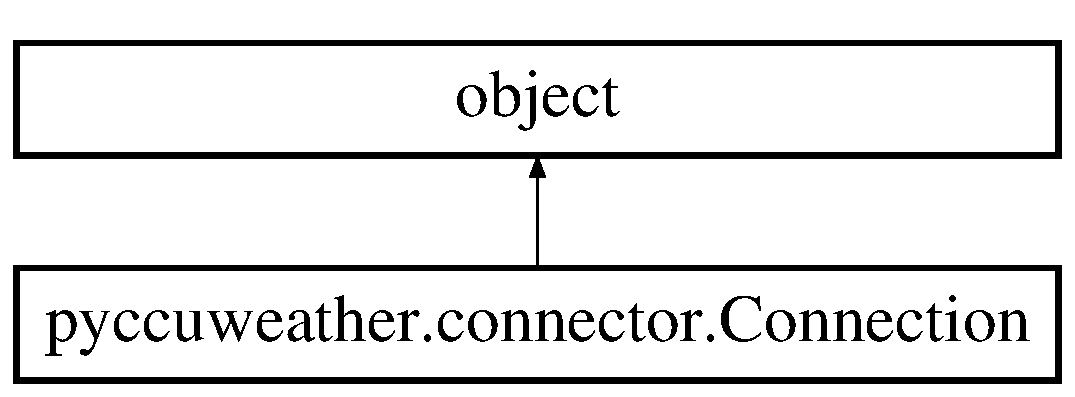
\includegraphics[height=2.000000cm]{classpyccuweather_1_1connector_1_1_connection}
\end{center}
\end{figure}
\subsection*{Public Member Functions}
\begin{DoxyCompactItemize}
\item 
\hypertarget{classpyccuweather_1_1connector_1_1_connection_a60b22d30224f352fb9125d258e83b82e}{}def {\bfseries \+\_\+\+\_\+init\+\_\+\+\_\+}\label{classpyccuweather_1_1connector_1_1_connection_a60b22d30224f352fb9125d258e83b82e}

\item 
\hypertarget{classpyccuweather_1_1connector_1_1_connection_afaa2776cf727065892230a1c65eb1c40}{}def {\bfseries \+\_\+\+\_\+str\+\_\+\+\_\+} (self)\label{classpyccuweather_1_1connector_1_1_connection_afaa2776cf727065892230a1c65eb1c40}

\item 
def \hyperlink{classpyccuweather_1_1connector_1_1_connection_afe5070f82e2ec598245b450a8c3e5b5e}{wipe\+\_\+api\+\_\+key} (self)
\item 
\hypertarget{classpyccuweather_1_1connector_1_1_connection_a3f389b4627b756a7d84f6840b71be8ad}{}def \hyperlink{classpyccuweather_1_1connector_1_1_connection_a3f389b4627b756a7d84f6840b71be8ad}{loc\+\_\+geoposition}\label{classpyccuweather_1_1connector_1_1_connection_a3f389b4627b756a7d84f6840b71be8ad}

\begin{DoxyCompactList}\small\item\em Location resolvers \#. \end{DoxyCompactList}\item 
\hypertarget{classpyccuweather_1_1connector_1_1_connection_a66e6990a0f54f43f7dea2d46beb6c070}{}def {\bfseries loc\+\_\+string}\label{classpyccuweather_1_1connector_1_1_connection_a66e6990a0f54f43f7dea2d46beb6c070}

\item 
\hypertarget{classpyccuweather_1_1connector_1_1_connection_aabac939e533b0881a8bf9534e70a57c4}{}def {\bfseries loc\+\_\+postcode}\label{classpyccuweather_1_1connector_1_1_connection_aabac939e533b0881a8bf9534e70a57c4}

\item 
\hypertarget{classpyccuweather_1_1connector_1_1_connection_aa60476694404266e2670be7569a2c40b}{}def {\bfseries loc\+\_\+ip}\label{classpyccuweather_1_1connector_1_1_connection_aa60476694404266e2670be7569a2c40b}

\item 
\hypertarget{classpyccuweather_1_1connector_1_1_connection_ae9321e2e564f7fc3ec74a6e543df8a33}{}def {\bfseries loc\+\_\+lkey}\label{classpyccuweather_1_1connector_1_1_connection_ae9321e2e564f7fc3ec74a6e543df8a33}

\item 
\hypertarget{classpyccuweather_1_1connector_1_1_connection_a726c54dac99acb74b26585d2f99af2b2}{}def \hyperlink{classpyccuweather_1_1connector_1_1_connection_a726c54dac99acb74b26585d2f99af2b2}{get\+\_\+current\+\_\+wx}\label{classpyccuweather_1_1connector_1_1_connection_a726c54dac99acb74b26585d2f99af2b2}

\begin{DoxyCompactList}\small\item\em Current conditions \#. \end{DoxyCompactList}\item 
\hypertarget{classpyccuweather_1_1connector_1_1_connection_a226bde67c9dad7db984365614e20c67a}{}def \hyperlink{classpyccuweather_1_1connector_1_1_connection_a226bde67c9dad7db984365614e20c67a}{get\+\_\+forecast}\label{classpyccuweather_1_1connector_1_1_connection_a226bde67c9dad7db984365614e20c67a}

\begin{DoxyCompactList}\small\item\em Forecasts \#. \end{DoxyCompactList}\item 
\hypertarget{classpyccuweather_1_1connector_1_1_connection_a8cc8445fce2183b2e3d1f36f36c3b104}{}def \hyperlink{classpyccuweather_1_1connector_1_1_connection_a8cc8445fce2183b2e3d1f36f36c3b104}{get\+\_\+airquality}\label{classpyccuweather_1_1connector_1_1_connection_a8cc8445fce2183b2e3d1f36f36c3b104}

\begin{DoxyCompactList}\small\item\em Air quality \#. \end{DoxyCompactList}\item 
\hypertarget{classpyccuweather_1_1connector_1_1_connection_a628bea15e42c2f23adc46021b69ea560}{}def \hyperlink{classpyccuweather_1_1connector_1_1_connection_a628bea15e42c2f23adc46021b69ea560}{get\+\_\+actuals}\label{classpyccuweather_1_1connector_1_1_connection_a628bea15e42c2f23adc46021b69ea560}

\begin{DoxyCompactList}\small\item\em Climo \#. \end{DoxyCompactList}\item 
\hypertarget{classpyccuweather_1_1connector_1_1_connection_abe7008dbe0600ac063c704d4780a5d46}{}def {\bfseries get\+\_\+records}\label{classpyccuweather_1_1connector_1_1_connection_abe7008dbe0600ac063c704d4780a5d46}

\item 
\hypertarget{classpyccuweather_1_1connector_1_1_connection_a5bca5ef6b2e462494948ae6d470bf4dd}{}def {\bfseries get\+\_\+normals}\label{classpyccuweather_1_1connector_1_1_connection_a5bca5ef6b2e462494948ae6d470bf4dd}

\item 
\hypertarget{classpyccuweather_1_1connector_1_1_connection_a23e9c86deb0e1234164aab99d6a765e7}{}def \hyperlink{classpyccuweather_1_1connector_1_1_connection_a23e9c86deb0e1234164aab99d6a765e7}{get\+\_\+alerts} (self, lkey, forecast\+\_\+range)\label{classpyccuweather_1_1connector_1_1_connection_a23e9c86deb0e1234164aab99d6a765e7}

\begin{DoxyCompactList}\small\item\em Alerts \#. \end{DoxyCompactList}\end{DoxyCompactItemize}
\subsection*{Public Attributes}
\begin{DoxyCompactItemize}
\item 
\hypertarget{classpyccuweather_1_1connector_1_1_connection_ab347ecfa9178e686fb17b8257fa612fa}{}{\bfseries A\+P\+I\+\_\+\+K\+E\+Y}\label{classpyccuweather_1_1connector_1_1_connection_ab347ecfa9178e686fb17b8257fa612fa}

\item 
\hypertarget{classpyccuweather_1_1connector_1_1_connection_a79bc370745ff57953bd5171d15d9730e}{}{\bfseries A\+P\+I\+\_\+\+R\+O\+O\+T}\label{classpyccuweather_1_1connector_1_1_connection_a79bc370745ff57953bd5171d15d9730e}

\item 
\hypertarget{classpyccuweather_1_1connector_1_1_connection_a5bbe33c3ad892efaec950ffd3d9e5b71}{}{\bfseries A\+P\+I\+\_\+\+V\+E\+R\+S\+I\+O\+N}\label{classpyccuweather_1_1connector_1_1_connection_a5bbe33c3ad892efaec950ffd3d9e5b71}

\item 
\hypertarget{classpyccuweather_1_1connector_1_1_connection_aaf21fd5e7b1adc7acaeaeb5700350513}{}{\bfseries retries}\label{classpyccuweather_1_1connector_1_1_connection_aaf21fd5e7b1adc7acaeaeb5700350513}

\end{DoxyCompactItemize}


\subsection{Detailed Description}
\begin{DoxyVerb}Represents a connection to the Accuweather API.

:param API_KEY: API key
:param dev: whether the dev mode api (apidev.accuweather.com) or the production api (api.accuweather.com) is used
:param retry: number of retries of failed operations - TODO: implement
:raise errors.MalformattedAPIKeyError: if the API key is not a 32-character string, an error is thrown
\end{DoxyVerb}
 

\subsection{Member Function Documentation}
\hypertarget{classpyccuweather_1_1connector_1_1_connection_afe5070f82e2ec598245b450a8c3e5b5e}{}\index{pyccuweather\+::connector\+::\+Connection@{pyccuweather\+::connector\+::\+Connection}!wipe\+\_\+api\+\_\+key@{wipe\+\_\+api\+\_\+key}}
\index{wipe\+\_\+api\+\_\+key@{wipe\+\_\+api\+\_\+key}!pyccuweather\+::connector\+::\+Connection@{pyccuweather\+::connector\+::\+Connection}}
\subsubsection[{wipe\+\_\+api\+\_\+key}]{\setlength{\rightskip}{0pt plus 5cm}def pyccuweather.\+connector.\+Connection.\+wipe\+\_\+api\+\_\+key (
\begin{DoxyParamCaption}
\item[{}]{self}
\end{DoxyParamCaption}
)}\label{classpyccuweather_1_1connector_1_1_connection_afe5070f82e2ec598245b450a8c3e5b5e}
\begin{DoxyVerb}Wipes API key from a Connection instance
:return: void
\end{DoxyVerb}
 

The documentation for this class was generated from the following file\+:\begin{DoxyCompactItemize}
\item 
pyccuweather/connector.\+py\end{DoxyCompactItemize}

\hypertarget{classpyccuweather_1_1objects_1_1_country}{}\section{pyccuweather.\+objects.\+Country Class Reference}
\label{classpyccuweather_1_1objects_1_1_country}\index{pyccuweather.\+objects.\+Country@{pyccuweather.\+objects.\+Country}}
Inheritance diagram for pyccuweather.\+objects.\+Country\+:\begin{figure}[H]
\begin{center}
\leavevmode
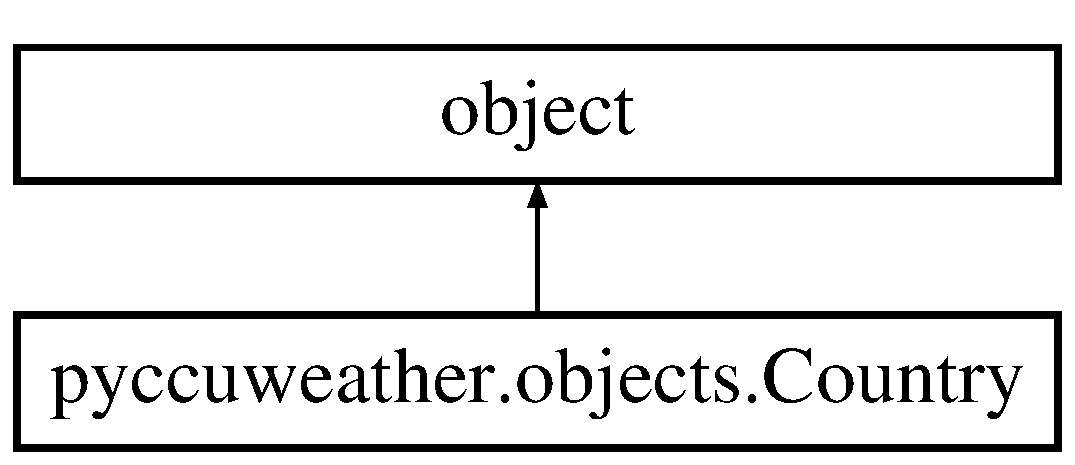
\includegraphics[height=2.000000cm]{classpyccuweather_1_1objects_1_1_country}
\end{center}
\end{figure}
\subsection*{Public Member Functions}
\begin{DoxyCompactItemize}
\item 
\hypertarget{classpyccuweather_1_1objects_1_1_country_a75be1bd9a2158a7fef301682d3c48454}{}def {\bfseries \+\_\+\+\_\+init\+\_\+\+\_\+}\label{classpyccuweather_1_1objects_1_1_country_a75be1bd9a2158a7fef301682d3c48454}

\item 
\hypertarget{classpyccuweather_1_1objects_1_1_country_ae2a347065c1d9072738e6a3d8042d5df}{}def {\bfseries \+\_\+\+\_\+str\+\_\+\+\_\+} (self)\label{classpyccuweather_1_1objects_1_1_country_ae2a347065c1d9072738e6a3d8042d5df}

\end{DoxyCompactItemize}
\subsection*{Public Attributes}
\begin{DoxyCompactItemize}
\item 
\hypertarget{classpyccuweather_1_1objects_1_1_country_a03f645bbf25c4cee40ebce2fdfc97215}{}{\bfseries id}\label{classpyccuweather_1_1objects_1_1_country_a03f645bbf25c4cee40ebce2fdfc97215}

\item 
\hypertarget{classpyccuweather_1_1objects_1_1_country_a7c6f624291a161173b4f306add66bd7d}{}{\bfseries localized\+\_\+name}\label{classpyccuweather_1_1objects_1_1_country_a7c6f624291a161173b4f306add66bd7d}

\item 
\hypertarget{classpyccuweather_1_1objects_1_1_country_a24f12c79057c8575fcfe52300f77de0f}{}{\bfseries english\+\_\+name}\label{classpyccuweather_1_1objects_1_1_country_a24f12c79057c8575fcfe52300f77de0f}

\end{DoxyCompactItemize}


\subsection{Detailed Description}
\begin{DoxyVerb}Represents a Country.
Countries are explained in the Accuweather documentation at http://apidev.accuweather.com/developers/countries
\end{DoxyVerb}
 

The documentation for this class was generated from the following file\+:\begin{DoxyCompactItemize}
\item 
pyccuweather/objects.\+py\end{DoxyCompactItemize}

\hypertarget{classpyccuweather_1_1objects_1_1_current_obs}{}\section{pyccuweather.\+objects.\+Current\+Obs Class Reference}
\label{classpyccuweather_1_1objects_1_1_current_obs}\index{pyccuweather.\+objects.\+Current\+Obs@{pyccuweather.\+objects.\+Current\+Obs}}
Inheritance diagram for pyccuweather.\+objects.\+Current\+Obs\+:\begin{figure}[H]
\begin{center}
\leavevmode
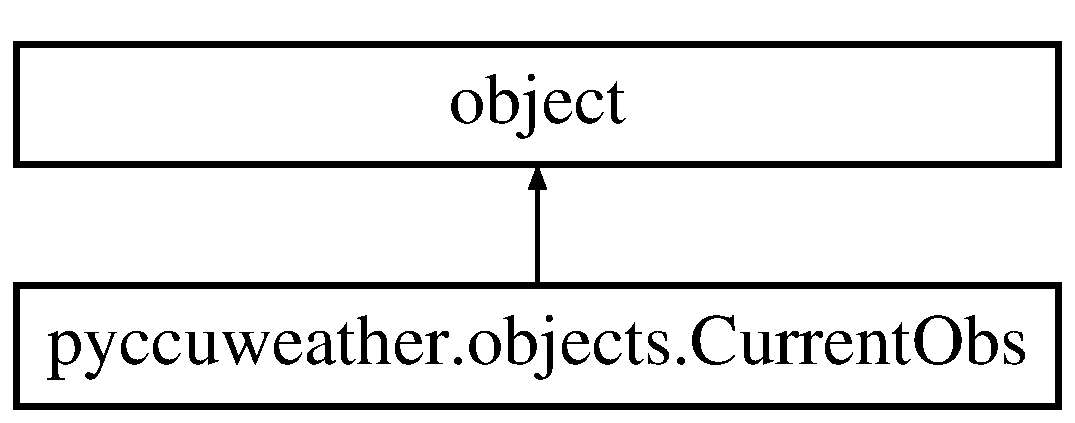
\includegraphics[height=2.000000cm]{classpyccuweather_1_1objects_1_1_current_obs}
\end{center}
\end{figure}
\subsection*{Public Member Functions}
\begin{DoxyCompactItemize}
\item 
\hypertarget{classpyccuweather_1_1objects_1_1_current_obs_afc5952bf9fd5841532045b281ed0e3b2}{}def {\bfseries \+\_\+\+\_\+init\+\_\+\+\_\+} (self, json)\label{classpyccuweather_1_1objects_1_1_current_obs_afc5952bf9fd5841532045b281ed0e3b2}

\item 
\hypertarget{classpyccuweather_1_1objects_1_1_current_obs_a4129560bbed935d0ba4710f8201d5ccd}{}def {\bfseries \+\_\+\+\_\+str\+\_\+\+\_\+} (self)\label{classpyccuweather_1_1objects_1_1_current_obs_a4129560bbed935d0ba4710f8201d5ccd}

\end{DoxyCompactItemize}
\subsection*{Public Attributes}
\begin{DoxyCompactItemize}
\item 
\hypertarget{classpyccuweather_1_1objects_1_1_current_obs_acf2488e0a0f0bcd9fd2d584fac16126d}{}{\bfseries observations}\label{classpyccuweather_1_1objects_1_1_current_obs_acf2488e0a0f0bcd9fd2d584fac16126d}

\item 
\hypertarget{classpyccuweather_1_1objects_1_1_current_obs_aaf9ce2cb50699fa70a4f5371acf5e531}{}{\bfseries raw}\label{classpyccuweather_1_1objects_1_1_current_obs_aaf9ce2cb50699fa70a4f5371acf5e531}

\end{DoxyCompactItemize}


The documentation for this class was generated from the following file\+:\begin{DoxyCompactItemize}
\item 
pyccuweather/objects.\+py\end{DoxyCompactItemize}

\hypertarget{classpyccuweather_1_1objects_1_1_daily_forecast}{}\section{pyccuweather.\+objects.\+Daily\+Forecast Class Reference}
\label{classpyccuweather_1_1objects_1_1_daily_forecast}\index{pyccuweather.\+objects.\+Daily\+Forecast@{pyccuweather.\+objects.\+Daily\+Forecast}}
Inheritance diagram for pyccuweather.\+objects.\+Daily\+Forecast\+:\begin{figure}[H]
\begin{center}
\leavevmode
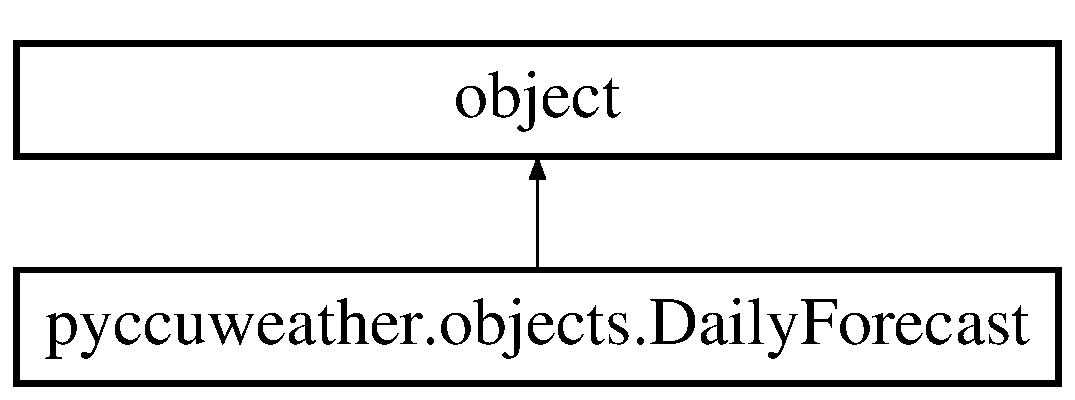
\includegraphics[height=2.000000cm]{classpyccuweather_1_1objects_1_1_daily_forecast}
\end{center}
\end{figure}
\subsection*{Public Member Functions}
\begin{DoxyCompactItemize}
\item 
\hypertarget{classpyccuweather_1_1objects_1_1_daily_forecast_a7591fefff1ddb8d49686b41c41c8da6a}{}def {\bfseries \+\_\+\+\_\+init\+\_\+\+\_\+} (self, json)\label{classpyccuweather_1_1objects_1_1_daily_forecast_a7591fefff1ddb8d49686b41c41c8da6a}

\item 
\hypertarget{classpyccuweather_1_1objects_1_1_daily_forecast_aa0b65f9fec13254b3b183e3fe284ba7b}{}def {\bfseries \+\_\+\+\_\+str\+\_\+\+\_\+} (self)\label{classpyccuweather_1_1objects_1_1_daily_forecast_aa0b65f9fec13254b3b183e3fe284ba7b}

\end{DoxyCompactItemize}
\subsection*{Public Attributes}
\begin{DoxyCompactItemize}
\item 
\hypertarget{classpyccuweather_1_1objects_1_1_daily_forecast_a14fe95921c66a9172d6a5a2863b442a9}{}{\bfseries epoch\+\_\+date}\label{classpyccuweather_1_1objects_1_1_daily_forecast_a14fe95921c66a9172d6a5a2863b442a9}

\item 
\hypertarget{classpyccuweather_1_1objects_1_1_daily_forecast_a54a70030577a671ccd766ab97d41eeba}{}{\bfseries date}\label{classpyccuweather_1_1objects_1_1_daily_forecast_a54a70030577a671ccd766ab97d41eeba}

\item 
\hypertarget{classpyccuweather_1_1objects_1_1_daily_forecast_a634923c021e9d7b73649ee2d6ae10a8f}{}{\bfseries temp\+\_\+min}\label{classpyccuweather_1_1objects_1_1_daily_forecast_a634923c021e9d7b73649ee2d6ae10a8f}

\item 
\hypertarget{classpyccuweather_1_1objects_1_1_daily_forecast_a2dbde530c3dcfb0051d6b25fb0318479}{}{\bfseries temp\+\_\+max}\label{classpyccuweather_1_1objects_1_1_daily_forecast_a2dbde530c3dcfb0051d6b25fb0318479}

\item 
\hypertarget{classpyccuweather_1_1objects_1_1_daily_forecast_a5ad1439ddd3ffb1b00a6c139c29a2be7}{}{\bfseries realfeel\+\_\+temp\+\_\+min}\label{classpyccuweather_1_1objects_1_1_daily_forecast_a5ad1439ddd3ffb1b00a6c139c29a2be7}

\item 
\hypertarget{classpyccuweather_1_1objects_1_1_daily_forecast_a95b6739049a11477902aa0cf935bec2b}{}{\bfseries realfeel\+\_\+temp\+\_\+max}\label{classpyccuweather_1_1objects_1_1_daily_forecast_a95b6739049a11477902aa0cf935bec2b}

\item 
\hypertarget{classpyccuweather_1_1objects_1_1_daily_forecast_a33c1c878bd7fa16906d8cfbeb05b8032}{}{\bfseries realfeel\+\_\+shade\+\_\+temp\+\_\+min}\label{classpyccuweather_1_1objects_1_1_daily_forecast_a33c1c878bd7fa16906d8cfbeb05b8032}

\item 
\hypertarget{classpyccuweather_1_1objects_1_1_daily_forecast_a41c4947bdac4e866a6ffcc4bbcf8cd6f}{}{\bfseries realfeel\+\_\+shade\+\_\+temp\+\_\+max}\label{classpyccuweather_1_1objects_1_1_daily_forecast_a41c4947bdac4e866a6ffcc4bbcf8cd6f}

\item 
\hypertarget{classpyccuweather_1_1objects_1_1_daily_forecast_acfe0799be4578d572e28306c6f4d8fd6}{}{\bfseries hours\+\_\+of\+\_\+sun}\label{classpyccuweather_1_1objects_1_1_daily_forecast_acfe0799be4578d572e28306c6f4d8fd6}

\item 
\hypertarget{classpyccuweather_1_1objects_1_1_daily_forecast_a999e2e41023f59bfb24b6b2c0dfaff8a}{}{\bfseries day}\label{classpyccuweather_1_1objects_1_1_daily_forecast_a999e2e41023f59bfb24b6b2c0dfaff8a}

\item 
\hypertarget{classpyccuweather_1_1objects_1_1_daily_forecast_a61bc6e78cbde2cf71986cca780bccaae}{}{\bfseries night}\label{classpyccuweather_1_1objects_1_1_daily_forecast_a61bc6e78cbde2cf71986cca780bccaae}

\item 
\hypertarget{classpyccuweather_1_1objects_1_1_daily_forecast_afdf04dd2429fd9eb41b5c8b5812582d3}{}{\bfseries raw}\label{classpyccuweather_1_1objects_1_1_daily_forecast_afdf04dd2429fd9eb41b5c8b5812582d3}

\end{DoxyCompactItemize}


The documentation for this class was generated from the following file\+:\begin{DoxyCompactItemize}
\item 
pyccuweather/objects.\+py\end{DoxyCompactItemize}

\hypertarget{classpyccuweather_1_1objects_1_1_daily_forecasts}{}\section{pyccuweather.\+objects.\+Daily\+Forecasts Class Reference}
\label{classpyccuweather_1_1objects_1_1_daily_forecasts}\index{pyccuweather.\+objects.\+Daily\+Forecasts@{pyccuweather.\+objects.\+Daily\+Forecasts}}
Inheritance diagram for pyccuweather.\+objects.\+Daily\+Forecasts\+:\begin{figure}[H]
\begin{center}
\leavevmode
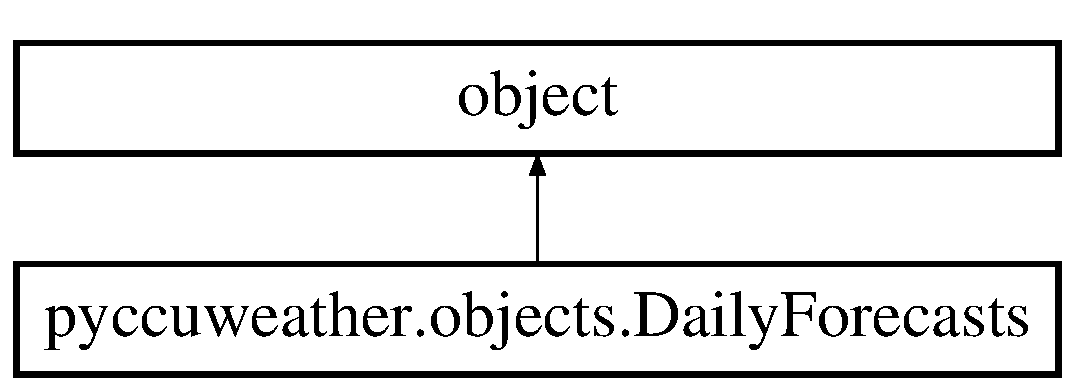
\includegraphics[height=2.000000cm]{classpyccuweather_1_1objects_1_1_daily_forecasts}
\end{center}
\end{figure}
\subsection*{Public Member Functions}
\begin{DoxyCompactItemize}
\item 
\hypertarget{classpyccuweather_1_1objects_1_1_daily_forecasts_a4ef14a31545197af17e376f261cf4ead}{}def {\bfseries \+\_\+\+\_\+init\+\_\+\+\_\+} (self, json)\label{classpyccuweather_1_1objects_1_1_daily_forecasts_a4ef14a31545197af17e376f261cf4ead}

\item 
\hypertarget{classpyccuweather_1_1objects_1_1_daily_forecasts_a58eead0280f9a9df67401de788adf7e2}{}def {\bfseries \+\_\+\+\_\+str\+\_\+\+\_\+} (self)\label{classpyccuweather_1_1objects_1_1_daily_forecasts_a58eead0280f9a9df67401de788adf7e2}

\end{DoxyCompactItemize}
\subsection*{Public Attributes}
\begin{DoxyCompactItemize}
\item 
\hypertarget{classpyccuweather_1_1objects_1_1_daily_forecasts_a09e2fe0933fba4e982258dfe890304d6}{}{\bfseries effective\+\_\+date}\label{classpyccuweather_1_1objects_1_1_daily_forecasts_a09e2fe0933fba4e982258dfe890304d6}

\item 
\hypertarget{classpyccuweather_1_1objects_1_1_daily_forecasts_aa031276990bf6f1d96c5e12d8e0ebf4d}{}{\bfseries effective\+\_\+epoch\+\_\+date}\label{classpyccuweather_1_1objects_1_1_daily_forecasts_aa031276990bf6f1d96c5e12d8e0ebf4d}

\item 
\hypertarget{classpyccuweather_1_1objects_1_1_daily_forecasts_aef969b946545dd22504b8f7034426ad8}{}{\bfseries end\+\_\+date}\label{classpyccuweather_1_1objects_1_1_daily_forecasts_aef969b946545dd22504b8f7034426ad8}

\item 
\hypertarget{classpyccuweather_1_1objects_1_1_daily_forecasts_aa1b15eaa58141994f4fe4937c066e130}{}{\bfseries end\+\_\+epoch\+\_\+date}\label{classpyccuweather_1_1objects_1_1_daily_forecasts_aa1b15eaa58141994f4fe4937c066e130}

\item 
\hypertarget{classpyccuweather_1_1objects_1_1_daily_forecasts_abaddf241e2251f918e8a9f04f6f0140c}{}{\bfseries severity}\label{classpyccuweather_1_1objects_1_1_daily_forecasts_abaddf241e2251f918e8a9f04f6f0140c}

\item 
\hypertarget{classpyccuweather_1_1objects_1_1_daily_forecasts_a52aef0531e08977cfd21923ef11f59f9}{}{\bfseries synopsis}\label{classpyccuweather_1_1objects_1_1_daily_forecasts_a52aef0531e08977cfd21923ef11f59f9}

\item 
\hypertarget{classpyccuweather_1_1objects_1_1_daily_forecasts_ad10804fd90a9d4d41e3f10f4a8781916}{}{\bfseries link}\label{classpyccuweather_1_1objects_1_1_daily_forecasts_ad10804fd90a9d4d41e3f10f4a8781916}

\item 
\hypertarget{classpyccuweather_1_1objects_1_1_daily_forecasts_a2534bd4513d41614840b4fbcb41bf67c}{}{\bfseries mobile\+\_\+link}\label{classpyccuweather_1_1objects_1_1_daily_forecasts_a2534bd4513d41614840b4fbcb41bf67c}

\item 
\hypertarget{classpyccuweather_1_1objects_1_1_daily_forecasts_a88957ab4a054c8080729a2df921fa159}{}{\bfseries forecasts}\label{classpyccuweather_1_1objects_1_1_daily_forecasts_a88957ab4a054c8080729a2df921fa159}

\item 
\hypertarget{classpyccuweather_1_1objects_1_1_daily_forecasts_aeee72fb67834c254e64f92f6f2a1ea8d}{}{\bfseries raw}\label{classpyccuweather_1_1objects_1_1_daily_forecasts_aeee72fb67834c254e64f92f6f2a1ea8d}

\end{DoxyCompactItemize}


The documentation for this class was generated from the following file\+:\begin{DoxyCompactItemize}
\item 
pyccuweather/objects.\+py\end{DoxyCompactItemize}

\hypertarget{classpyccuweather_1_1objects_1_1_degree_day}{}\section{pyccuweather.\+objects.\+Degree\+Day Class Reference}
\label{classpyccuweather_1_1objects_1_1_degree_day}\index{pyccuweather.\+objects.\+Degree\+Day@{pyccuweather.\+objects.\+Degree\+Day}}
Inheritance diagram for pyccuweather.\+objects.\+Degree\+Day\+:\begin{figure}[H]
\begin{center}
\leavevmode
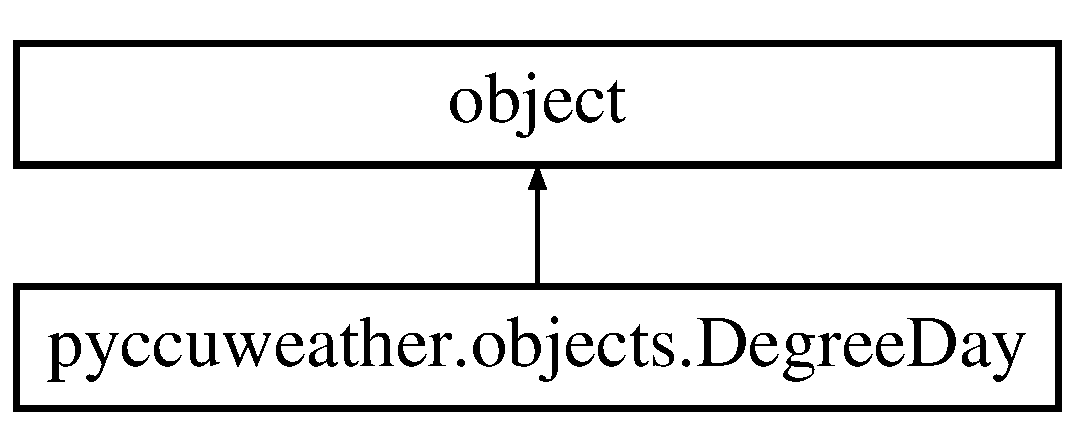
\includegraphics[height=2.000000cm]{classpyccuweather_1_1objects_1_1_degree_day}
\end{center}
\end{figure}
\subsection*{Public Member Functions}
\begin{DoxyCompactItemize}
\item 
\hypertarget{classpyccuweather_1_1objects_1_1_degree_day_aa2ed6f5e809e02d62930362936f8a1e1}{}def {\bfseries \+\_\+\+\_\+init\+\_\+\+\_\+} (self, aqf\+\_\+dict)\label{classpyccuweather_1_1objects_1_1_degree_day_aa2ed6f5e809e02d62930362936f8a1e1}

\end{DoxyCompactItemize}
\subsection*{Public Attributes}
\begin{DoxyCompactItemize}
\item 
\hypertarget{classpyccuweather_1_1objects_1_1_degree_day_a8ca968ca5dc856235a9c5e3f1fdc9b1b}{}{\bfseries cooling}\label{classpyccuweather_1_1objects_1_1_degree_day_a8ca968ca5dc856235a9c5e3f1fdc9b1b}

\item 
\hypertarget{classpyccuweather_1_1objects_1_1_degree_day_a3aeb2a2c2a4e1c95688c95ab7c383b58}{}{\bfseries warming}\label{classpyccuweather_1_1objects_1_1_degree_day_a3aeb2a2c2a4e1c95688c95ab7c383b58}

\end{DoxyCompactItemize}


The documentation for this class was generated from the following file\+:\begin{DoxyCompactItemize}
\item 
pyccuweather/objects.\+py\end{DoxyCompactItemize}

\hypertarget{classpyccuweather_1_1objects_1_1_hemiurnal}{}\section{pyccuweather.\+objects.\+Hemiurnal Class Reference}
\label{classpyccuweather_1_1objects_1_1_hemiurnal}\index{pyccuweather.\+objects.\+Hemiurnal@{pyccuweather.\+objects.\+Hemiurnal}}
Inheritance diagram for pyccuweather.\+objects.\+Hemiurnal\+:\begin{figure}[H]
\begin{center}
\leavevmode
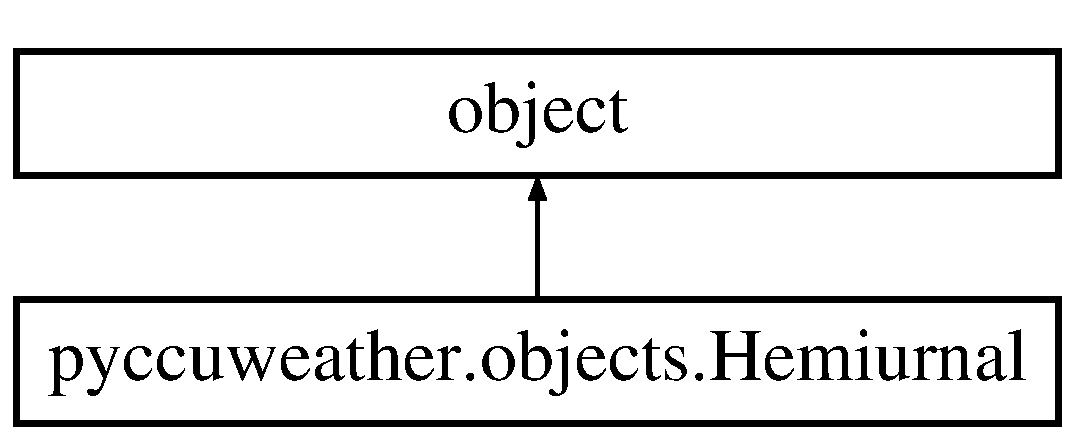
\includegraphics[height=2.000000cm]{classpyccuweather_1_1objects_1_1_hemiurnal}
\end{center}
\end{figure}
\subsection*{Public Member Functions}
\begin{DoxyCompactItemize}
\item 
\hypertarget{classpyccuweather_1_1objects_1_1_hemiurnal_acbdbb672259d2dd0ac557fa389aea6b0}{}def {\bfseries \+\_\+\+\_\+init\+\_\+\+\_\+} (self, json)\label{classpyccuweather_1_1objects_1_1_hemiurnal_acbdbb672259d2dd0ac557fa389aea6b0}

\item 
\hypertarget{classpyccuweather_1_1objects_1_1_hemiurnal_a7b1e66a5d2639f21b6718193a0628573}{}def {\bfseries \+\_\+\+\_\+str\+\_\+\+\_\+} (self)\label{classpyccuweather_1_1objects_1_1_hemiurnal_a7b1e66a5d2639f21b6718193a0628573}

\end{DoxyCompactItemize}
\subsection*{Public Attributes}
\begin{DoxyCompactItemize}
\item 
\hypertarget{classpyccuweather_1_1objects_1_1_hemiurnal_a963c10caec1c965b870759259b78694a}{}{\bfseries id}\label{classpyccuweather_1_1objects_1_1_hemiurnal_a963c10caec1c965b870759259b78694a}

\item 
\hypertarget{classpyccuweather_1_1objects_1_1_hemiurnal_a0b66e85bcadda8fd200d169cb02ef547}{}{\bfseries synopsis}\label{classpyccuweather_1_1objects_1_1_hemiurnal_a0b66e85bcadda8fd200d169cb02ef547}

\item 
\hypertarget{classpyccuweather_1_1objects_1_1_hemiurnal_a89022f3c47dcafdcee59b785f34381dd}{}{\bfseries phrase}\label{classpyccuweather_1_1objects_1_1_hemiurnal_a89022f3c47dcafdcee59b785f34381dd}

\item 
\hypertarget{classpyccuweather_1_1objects_1_1_hemiurnal_af3accdb2dbe8cf170f43de063edb151f}{}{\bfseries snow}\label{classpyccuweather_1_1objects_1_1_hemiurnal_af3accdb2dbe8cf170f43de063edb151f}

\item 
\hypertarget{classpyccuweather_1_1objects_1_1_hemiurnal_a944a6340184bc7b261b672c6d25f6586}{}{\bfseries wind}\label{classpyccuweather_1_1objects_1_1_hemiurnal_a944a6340184bc7b261b672c6d25f6586}

\item 
\hypertarget{classpyccuweather_1_1objects_1_1_hemiurnal_a39ce023a1f8ff37ec769d5f61141d38b}{}{\bfseries rain}\label{classpyccuweather_1_1objects_1_1_hemiurnal_a39ce023a1f8ff37ec769d5f61141d38b}

\item 
\hypertarget{classpyccuweather_1_1objects_1_1_hemiurnal_a360bb9600f3b1c7405040fa2584aa007}{}{\bfseries ice}\label{classpyccuweather_1_1objects_1_1_hemiurnal_a360bb9600f3b1c7405040fa2584aa007}

\item 
\hypertarget{classpyccuweather_1_1objects_1_1_hemiurnal_a18365ce791193ea9158c5e884c001141}{}{\bfseries total\+\_\+liquid}\label{classpyccuweather_1_1objects_1_1_hemiurnal_a18365ce791193ea9158c5e884c001141}

\item 
\hypertarget{classpyccuweather_1_1objects_1_1_hemiurnal_a78d83d56d05e84b733308efa58b26b25}{}{\bfseries h\+\_\+precipitation}\label{classpyccuweather_1_1objects_1_1_hemiurnal_a78d83d56d05e84b733308efa58b26b25}

\item 
\hypertarget{classpyccuweather_1_1objects_1_1_hemiurnal_adbd1f190ab5134cdccd4bf34d2c1c3e9}{}{\bfseries h\+\_\+rain}\label{classpyccuweather_1_1objects_1_1_hemiurnal_adbd1f190ab5134cdccd4bf34d2c1c3e9}

\item 
\hypertarget{classpyccuweather_1_1objects_1_1_hemiurnal_a917d2c35ca9196b9767ac7c49390ce63}{}{\bfseries cloud\+\_\+cover}\label{classpyccuweather_1_1objects_1_1_hemiurnal_a917d2c35ca9196b9767ac7c49390ce63}

\item 
\hypertarget{classpyccuweather_1_1objects_1_1_hemiurnal_ae2179180bffc08a06a074bc7073342d2}{}{\bfseries p\+\_\+rain}\label{classpyccuweather_1_1objects_1_1_hemiurnal_ae2179180bffc08a06a074bc7073342d2}

\item 
\hypertarget{classpyccuweather_1_1objects_1_1_hemiurnal_a93fefe1768bfc0f31a71103571e8cb8d}{}{\bfseries p\+\_\+snow}\label{classpyccuweather_1_1objects_1_1_hemiurnal_a93fefe1768bfc0f31a71103571e8cb8d}

\item 
\hypertarget{classpyccuweather_1_1objects_1_1_hemiurnal_a6a1ab6daa88ae5ac9bab73f278f7dc8b}{}{\bfseries p\+\_\+ice}\label{classpyccuweather_1_1objects_1_1_hemiurnal_a6a1ab6daa88ae5ac9bab73f278f7dc8b}

\item 
\hypertarget{classpyccuweather_1_1objects_1_1_hemiurnal_a5a2a7d678c742151f7f163648317489d}{}{\bfseries p\+\_\+thunderstorm}\label{classpyccuweather_1_1objects_1_1_hemiurnal_a5a2a7d678c742151f7f163648317489d}

\item 
\hypertarget{classpyccuweather_1_1objects_1_1_hemiurnal_af0ba559638fa22de1cba1e0ca5c749ac}{}{\bfseries p\+\_\+precipitation}\label{classpyccuweather_1_1objects_1_1_hemiurnal_af0ba559638fa22de1cba1e0ca5c749ac}

\item 
\hypertarget{classpyccuweather_1_1objects_1_1_hemiurnal_a4ad05c068544cf2c018092f49c84029b}{}{\bfseries wind\+\_\+gust}\label{classpyccuweather_1_1objects_1_1_hemiurnal_a4ad05c068544cf2c018092f49c84029b}

\item 
\hypertarget{classpyccuweather_1_1objects_1_1_hemiurnal_a4b06823bf078385305e2c54a7fa0db09}{}{\bfseries raw}\label{classpyccuweather_1_1objects_1_1_hemiurnal_a4b06823bf078385305e2c54a7fa0db09}

\end{DoxyCompactItemize}


The documentation for this class was generated from the following file\+:\begin{DoxyCompactItemize}
\item 
pyccuweather/objects.\+py\end{DoxyCompactItemize}

\hypertarget{classpyccuweather_1_1objects_1_1_hourly_forecast}{}\section{pyccuweather.\+objects.\+Hourly\+Forecast Class Reference}
\label{classpyccuweather_1_1objects_1_1_hourly_forecast}\index{pyccuweather.\+objects.\+Hourly\+Forecast@{pyccuweather.\+objects.\+Hourly\+Forecast}}
Inheritance diagram for pyccuweather.\+objects.\+Hourly\+Forecast\+:\begin{figure}[H]
\begin{center}
\leavevmode
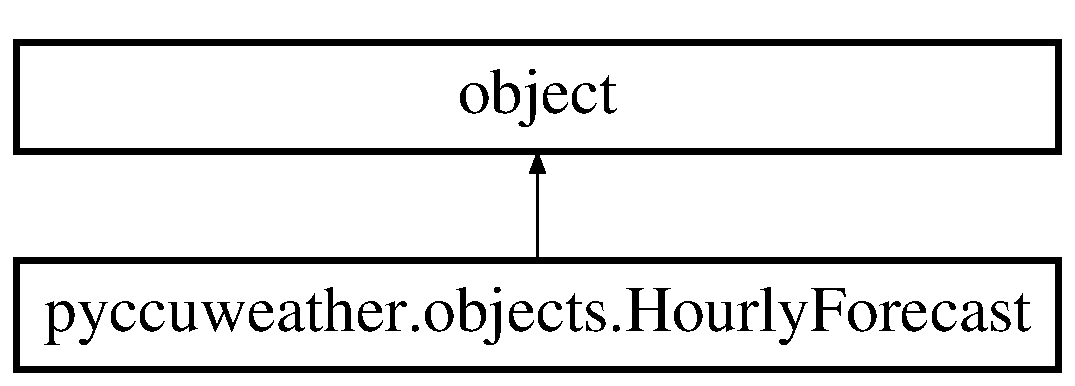
\includegraphics[height=2.000000cm]{classpyccuweather_1_1objects_1_1_hourly_forecast}
\end{center}
\end{figure}
\subsection*{Public Member Functions}
\begin{DoxyCompactItemize}
\item 
\hypertarget{classpyccuweather_1_1objects_1_1_hourly_forecast_a42c16958d6739bef3dc896794af3845b}{}def {\bfseries \+\_\+\+\_\+init\+\_\+\+\_\+} (self, json)\label{classpyccuweather_1_1objects_1_1_hourly_forecast_a42c16958d6739bef3dc896794af3845b}

\item 
\hypertarget{classpyccuweather_1_1objects_1_1_hourly_forecast_ae814906e26d967ce0f90f020de774dd2}{}def {\bfseries \+\_\+\+\_\+str\+\_\+\+\_\+} (self)\label{classpyccuweather_1_1objects_1_1_hourly_forecast_ae814906e26d967ce0f90f020de774dd2}

\end{DoxyCompactItemize}
\subsection*{Public Attributes}
\begin{DoxyCompactItemize}
\item 
\hypertarget{classpyccuweather_1_1objects_1_1_hourly_forecast_a0577a949cea16ab415d94da239615e83}{}{\bfseries epoch\+\_\+datetime}\label{classpyccuweather_1_1objects_1_1_hourly_forecast_a0577a949cea16ab415d94da239615e83}

\item 
\hypertarget{classpyccuweather_1_1objects_1_1_hourly_forecast_aef71cf8e54c8247ee141f483c820e7ef}{}{\bfseries datetime}\label{classpyccuweather_1_1objects_1_1_hourly_forecast_aef71cf8e54c8247ee141f483c820e7ef}

\item 
\hypertarget{classpyccuweather_1_1objects_1_1_hourly_forecast_a1e0aa3c8bb2155414cb115823d9ac552}{}{\bfseries temperature}\label{classpyccuweather_1_1objects_1_1_hourly_forecast_a1e0aa3c8bb2155414cb115823d9ac552}

\item 
\hypertarget{classpyccuweather_1_1objects_1_1_hourly_forecast_a53b0efde0400759375938845553f9bf7}{}{\bfseries realfeel\+\_\+temperature}\label{classpyccuweather_1_1objects_1_1_hourly_forecast_a53b0efde0400759375938845553f9bf7}

\item 
\hypertarget{classpyccuweather_1_1objects_1_1_hourly_forecast_a44edbfa5e8e0c06211d51d5a2ff44874}{}{\bfseries cloud\+\_\+cover}\label{classpyccuweather_1_1objects_1_1_hourly_forecast_a44edbfa5e8e0c06211d51d5a2ff44874}

\item 
\hypertarget{classpyccuweather_1_1objects_1_1_hourly_forecast_ae184f775300f91fe9ea2da193e2febf1}{}{\bfseries ceiling}\label{classpyccuweather_1_1objects_1_1_hourly_forecast_ae184f775300f91fe9ea2da193e2febf1}

\item 
\hypertarget{classpyccuweather_1_1objects_1_1_hourly_forecast_ac54cb42e4fdbebdcd9d4325f3bddff4a}{}{\bfseries wind}\label{classpyccuweather_1_1objects_1_1_hourly_forecast_ac54cb42e4fdbebdcd9d4325f3bddff4a}

\item 
\hypertarget{classpyccuweather_1_1objects_1_1_hourly_forecast_aa5529484b29e1a79ac02501d22ce7b9b}{}{\bfseries wind\+\_\+gust}\label{classpyccuweather_1_1objects_1_1_hourly_forecast_aa5529484b29e1a79ac02501d22ce7b9b}

\item 
\hypertarget{classpyccuweather_1_1objects_1_1_hourly_forecast_ad08b94b75593e154ddf7b2f5d4256fdc}{}{\bfseries rh}\label{classpyccuweather_1_1objects_1_1_hourly_forecast_ad08b94b75593e154ddf7b2f5d4256fdc}

\item 
\hypertarget{classpyccuweather_1_1objects_1_1_hourly_forecast_a3681340329d90cde05c4c01478afed5a}{}{\bfseries dewpoint}\label{classpyccuweather_1_1objects_1_1_hourly_forecast_a3681340329d90cde05c4c01478afed5a}

\item 
\hypertarget{classpyccuweather_1_1objects_1_1_hourly_forecast_a9dfa6f9729355fdc8eed838dd02c924e}{}{\bfseries wet\+\_\+bulb\+\_\+temperature}\label{classpyccuweather_1_1objects_1_1_hourly_forecast_a9dfa6f9729355fdc8eed838dd02c924e}

\item 
\hypertarget{classpyccuweather_1_1objects_1_1_hourly_forecast_aa1a26005e415ae02858c0cd5afab501f}{}{\bfseries uv\+\_\+index}\label{classpyccuweather_1_1objects_1_1_hourly_forecast_aa1a26005e415ae02858c0cd5afab501f}

\item 
\hypertarget{classpyccuweather_1_1objects_1_1_hourly_forecast_a2c1764eb593a0f608f070f1cb97875a1}{}{\bfseries uv\+\_\+index\+\_\+text}\label{classpyccuweather_1_1objects_1_1_hourly_forecast_a2c1764eb593a0f608f070f1cb97875a1}

\item 
\hypertarget{classpyccuweather_1_1objects_1_1_hourly_forecast_a27186232ce81c8e80d397dfb942fd291}{}{\bfseries rain}\label{classpyccuweather_1_1objects_1_1_hourly_forecast_a27186232ce81c8e80d397dfb942fd291}

\item 
\hypertarget{classpyccuweather_1_1objects_1_1_hourly_forecast_a15ad1354fdeccac0bd18336a06472fae}{}{\bfseries total\+\_\+liquid}\label{classpyccuweather_1_1objects_1_1_hourly_forecast_a15ad1354fdeccac0bd18336a06472fae}

\item 
\hypertarget{classpyccuweather_1_1objects_1_1_hourly_forecast_a002263f3cadbeac9f931dc8c6e382ce9}{}{\bfseries ice}\label{classpyccuweather_1_1objects_1_1_hourly_forecast_a002263f3cadbeac9f931dc8c6e382ce9}

\item 
\hypertarget{classpyccuweather_1_1objects_1_1_hourly_forecast_a1e28ec4afe4268e14e01923dda745147}{}{\bfseries snow}\label{classpyccuweather_1_1objects_1_1_hourly_forecast_a1e28ec4afe4268e14e01923dda745147}

\item 
\hypertarget{classpyccuweather_1_1objects_1_1_hourly_forecast_a36be9493393145fa16e192fe94774f5d}{}{\bfseries p\+\_\+snow}\label{classpyccuweather_1_1objects_1_1_hourly_forecast_a36be9493393145fa16e192fe94774f5d}

\item 
\hypertarget{classpyccuweather_1_1objects_1_1_hourly_forecast_a77d246511314edaa8021c8114cd90e10}{}{\bfseries p\+\_\+ice}\label{classpyccuweather_1_1objects_1_1_hourly_forecast_a77d246511314edaa8021c8114cd90e10}

\item 
\hypertarget{classpyccuweather_1_1objects_1_1_hourly_forecast_a2c155addb274309204488e368811cf16}{}{\bfseries p\+\_\+rain}\label{classpyccuweather_1_1objects_1_1_hourly_forecast_a2c155addb274309204488e368811cf16}

\item 
\hypertarget{classpyccuweather_1_1objects_1_1_hourly_forecast_a09c7ffa018743d902c8473e73b88c40a}{}{\bfseries p\+\_\+precipitation}\label{classpyccuweather_1_1objects_1_1_hourly_forecast_a09c7ffa018743d902c8473e73b88c40a}

\item 
\hypertarget{classpyccuweather_1_1objects_1_1_hourly_forecast_acfa95a8f4af257330b5011e954721852}{}{\bfseries link}\label{classpyccuweather_1_1objects_1_1_hourly_forecast_acfa95a8f4af257330b5011e954721852}

\item 
\hypertarget{classpyccuweather_1_1objects_1_1_hourly_forecast_a84f6ad0af8af412bb8f717c853248507}{}{\bfseries mobile\+\_\+link}\label{classpyccuweather_1_1objects_1_1_hourly_forecast_a84f6ad0af8af412bb8f717c853248507}

\item 
\hypertarget{classpyccuweather_1_1objects_1_1_hourly_forecast_a40177f73dc2078e640b90ed96f20226f}{}{\bfseries raw}\label{classpyccuweather_1_1objects_1_1_hourly_forecast_a40177f73dc2078e640b90ed96f20226f}

\end{DoxyCompactItemize}


The documentation for this class was generated from the following file\+:\begin{DoxyCompactItemize}
\item 
pyccuweather/objects.\+py\end{DoxyCompactItemize}

\hypertarget{classpyccuweather_1_1objects_1_1_hourly_forecasts}{}\section{pyccuweather.\+objects.\+Hourly\+Forecasts Class Reference}
\label{classpyccuweather_1_1objects_1_1_hourly_forecasts}\index{pyccuweather.\+objects.\+Hourly\+Forecasts@{pyccuweather.\+objects.\+Hourly\+Forecasts}}
Inheritance diagram for pyccuweather.\+objects.\+Hourly\+Forecasts\+:\begin{figure}[H]
\begin{center}
\leavevmode
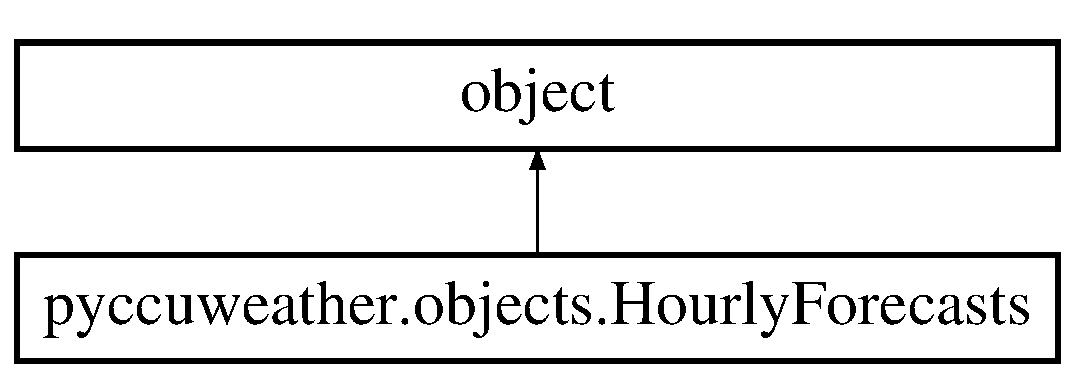
\includegraphics[height=2.000000cm]{classpyccuweather_1_1objects_1_1_hourly_forecasts}
\end{center}
\end{figure}
\subsection*{Public Member Functions}
\begin{DoxyCompactItemize}
\item 
\hypertarget{classpyccuweather_1_1objects_1_1_hourly_forecasts_afae877cc383a552a49bd4dc45314b7f3}{}def {\bfseries \+\_\+\+\_\+init\+\_\+\+\_\+} (self, json)\label{classpyccuweather_1_1objects_1_1_hourly_forecasts_afae877cc383a552a49bd4dc45314b7f3}

\item 
\hypertarget{classpyccuweather_1_1objects_1_1_hourly_forecasts_a892f7098c8b4bfcdfebff293fa3a794e}{}def {\bfseries \+\_\+\+\_\+str\+\_\+\+\_\+} (self)\label{classpyccuweather_1_1objects_1_1_hourly_forecasts_a892f7098c8b4bfcdfebff293fa3a794e}

\end{DoxyCompactItemize}
\subsection*{Public Attributes}
\begin{DoxyCompactItemize}
\item 
\hypertarget{classpyccuweather_1_1objects_1_1_hourly_forecasts_aff5bd0d411a9b37e016ee4c786721c24}{}{\bfseries forecasts}\label{classpyccuweather_1_1objects_1_1_hourly_forecasts_aff5bd0d411a9b37e016ee4c786721c24}

\item 
\hypertarget{classpyccuweather_1_1objects_1_1_hourly_forecasts_ad4274d81a2ede68449839fcdc9c5cb37}{}{\bfseries raw}\label{classpyccuweather_1_1objects_1_1_hourly_forecasts_ad4274d81a2ede68449839fcdc9c5cb37}

\end{DoxyCompactItemize}


The documentation for this class was generated from the following file\+:\begin{DoxyCompactItemize}
\item 
pyccuweather/objects.\+py\end{DoxyCompactItemize}

\hypertarget{classpyccuweather_1_1errors_1_1_invalid_country_code_error}{}\section{pyccuweather.\+errors.\+Invalid\+Country\+Code\+Error Class Reference}
\label{classpyccuweather_1_1errors_1_1_invalid_country_code_error}\index{pyccuweather.\+errors.\+Invalid\+Country\+Code\+Error@{pyccuweather.\+errors.\+Invalid\+Country\+Code\+Error}}
Inheritance diagram for pyccuweather.\+errors.\+Invalid\+Country\+Code\+Error\+:\begin{figure}[H]
\begin{center}
\leavevmode
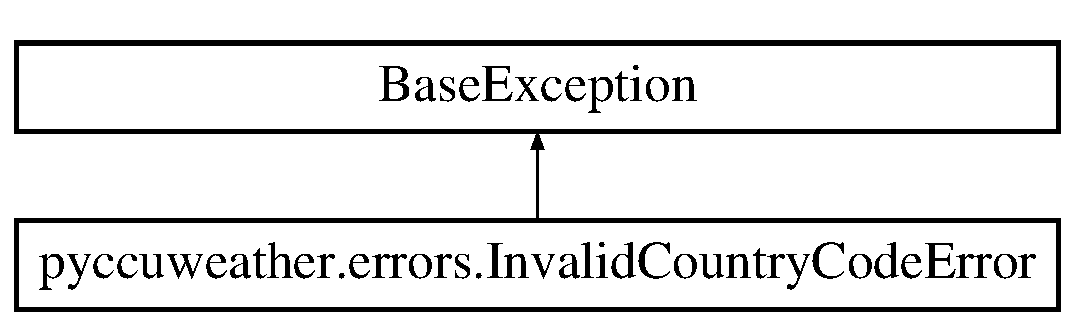
\includegraphics[height=2.000000cm]{classpyccuweather_1_1errors_1_1_invalid_country_code_error}
\end{center}
\end{figure}
\subsection*{Public Member Functions}
\begin{DoxyCompactItemize}
\item 
\hypertarget{classpyccuweather_1_1errors_1_1_invalid_country_code_error_ab9100d4e149370b99bddc201c5d0d5c9}{}def {\bfseries \+\_\+\+\_\+init\+\_\+\+\_\+} (self, country\+\_\+code)\label{classpyccuweather_1_1errors_1_1_invalid_country_code_error_ab9100d4e149370b99bddc201c5d0d5c9}

\item 
\hypertarget{classpyccuweather_1_1errors_1_1_invalid_country_code_error_a4307b904b12b319a8ae67bb54037a9f6}{}def {\bfseries \+\_\+\+\_\+str\+\_\+\+\_\+} (self)\label{classpyccuweather_1_1errors_1_1_invalid_country_code_error_a4307b904b12b319a8ae67bb54037a9f6}

\end{DoxyCompactItemize}
\subsection*{Public Attributes}
\begin{DoxyCompactItemize}
\item 
\hypertarget{classpyccuweather_1_1errors_1_1_invalid_country_code_error_abfb5f3a1ced80e452db7360661a442ca}{}{\bfseries country\+\_\+code}\label{classpyccuweather_1_1errors_1_1_invalid_country_code_error_abfb5f3a1ced80e452db7360661a442ca}

\end{DoxyCompactItemize}


\subsection{Detailed Description}
\begin{DoxyVerb}Raised when a country code is provided that does not exist.
Valid country codes are listed by Accuweather under http://apidev.accuweather.com/developers/countries
\end{DoxyVerb}
 

The documentation for this class was generated from the following file\+:\begin{DoxyCompactItemize}
\item 
pyccuweather/errors.\+py\end{DoxyCompactItemize}

\hypertarget{classpyccuweather_1_1objects_1_1_location}{}\section{pyccuweather.\+objects.\+Location Class Reference}
\label{classpyccuweather_1_1objects_1_1_location}\index{pyccuweather.\+objects.\+Location@{pyccuweather.\+objects.\+Location}}
Inheritance diagram for pyccuweather.\+objects.\+Location\+:\begin{figure}[H]
\begin{center}
\leavevmode
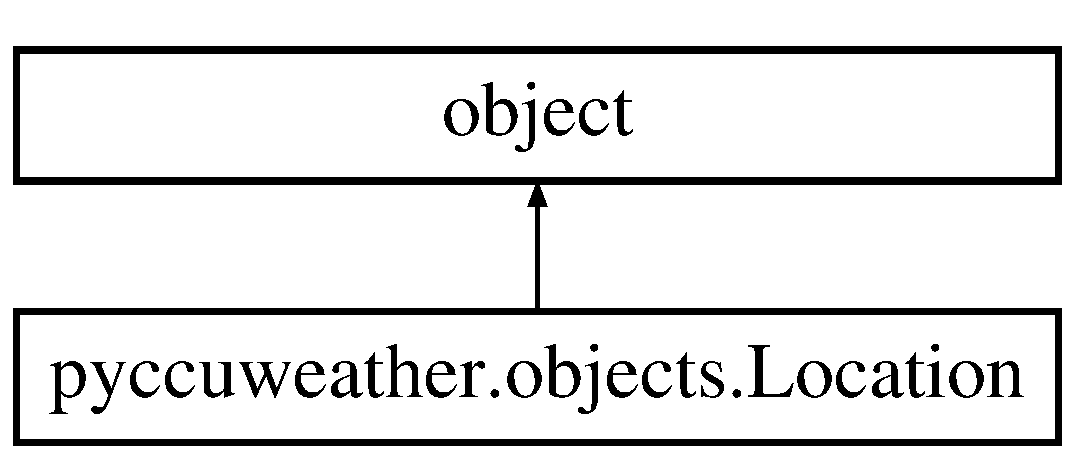
\includegraphics[height=2.000000cm]{classpyccuweather_1_1objects_1_1_location}
\end{center}
\end{figure}
\subsection*{Public Member Functions}
\begin{DoxyCompactItemize}
\item 
\hypertarget{classpyccuweather_1_1objects_1_1_location_aa3a11864142d6d0ed0e0648de21a4bf6}{}def {\bfseries \+\_\+\+\_\+init\+\_\+\+\_\+}\label{classpyccuweather_1_1objects_1_1_location_aa3a11864142d6d0ed0e0648de21a4bf6}

\item 
\hypertarget{classpyccuweather_1_1objects_1_1_location_abd73ef019b1c5216b5df298dee0ac9ad}{}def {\bfseries \+\_\+\+\_\+str\+\_\+\+\_\+} (self)\label{classpyccuweather_1_1objects_1_1_location_abd73ef019b1c5216b5df298dee0ac9ad}

\end{DoxyCompactItemize}
\subsection*{Public Attributes}
\begin{DoxyCompactItemize}
\item 
\hypertarget{classpyccuweather_1_1objects_1_1_location_a2db9c266ed0f1cda6697323ce4bf3c66}{}{\bfseries lkey}\label{classpyccuweather_1_1objects_1_1_location_a2db9c266ed0f1cda6697323ce4bf3c66}

\item 
\hypertarget{classpyccuweather_1_1objects_1_1_location_a741c75c01dd100be1dfb7cd319c5859b}{}{\bfseries lat}\label{classpyccuweather_1_1objects_1_1_location_a741c75c01dd100be1dfb7cd319c5859b}

\item 
\hypertarget{classpyccuweather_1_1objects_1_1_location_a0f4e42a2f859242d37b9542081dc29df}{}{\bfseries lon}\label{classpyccuweather_1_1objects_1_1_location_a0f4e42a2f859242d37b9542081dc29df}

\item 
\hypertarget{classpyccuweather_1_1objects_1_1_location_aa9f23fbb86e84a0c23be2c50a46cb8db}{}{\bfseries localized\+\_\+name}\label{classpyccuweather_1_1objects_1_1_location_aa9f23fbb86e84a0c23be2c50a46cb8db}

\item 
\hypertarget{classpyccuweather_1_1objects_1_1_location_abf629be0339a33b0092231af44eae4e2}{}{\bfseries english\+\_\+name}\label{classpyccuweather_1_1objects_1_1_location_abf629be0339a33b0092231af44eae4e2}

\item 
\hypertarget{classpyccuweather_1_1objects_1_1_location_a8d5c854db6a2f9971bfbf7597ea448f9}{}{\bfseries region}\label{classpyccuweather_1_1objects_1_1_location_a8d5c854db6a2f9971bfbf7597ea448f9}

\item 
\hypertarget{classpyccuweather_1_1objects_1_1_location_a495204cb84378865bed79dc18557dfa3}{}{\bfseries country}\label{classpyccuweather_1_1objects_1_1_location_a495204cb84378865bed79dc18557dfa3}

\item 
\hypertarget{classpyccuweather_1_1objects_1_1_location_a65bcffd46c1c16d42b042b0db62ff525}{}{\bfseries administrative\+\_\+area}\label{classpyccuweather_1_1objects_1_1_location_a65bcffd46c1c16d42b042b0db62ff525}

\item 
\hypertarget{classpyccuweather_1_1objects_1_1_location_a00a6fbdd23b35c42f97da8befcbe4943}{}{\bfseries timezone}\label{classpyccuweather_1_1objects_1_1_location_a00a6fbdd23b35c42f97da8befcbe4943}

\end{DoxyCompactItemize}


\subsection{Detailed Description}
\begin{DoxyVerb}Represents a Location.
Locations are explained in the Accuweather documentation at http://apidev.accuweather.com/developers/locations
\end{DoxyVerb}
 

The documentation for this class was generated from the following file\+:\begin{DoxyCompactItemize}
\item 
pyccuweather/objects.\+py\end{DoxyCompactItemize}

\hypertarget{classpyccuweather_1_1objects_1_1_location_set}{}\section{pyccuweather.\+objects.\+Location\+Set Class Reference}
\label{classpyccuweather_1_1objects_1_1_location_set}\index{pyccuweather.\+objects.\+Location\+Set@{pyccuweather.\+objects.\+Location\+Set}}
Inheritance diagram for pyccuweather.\+objects.\+Location\+Set\+:\begin{figure}[H]
\begin{center}
\leavevmode
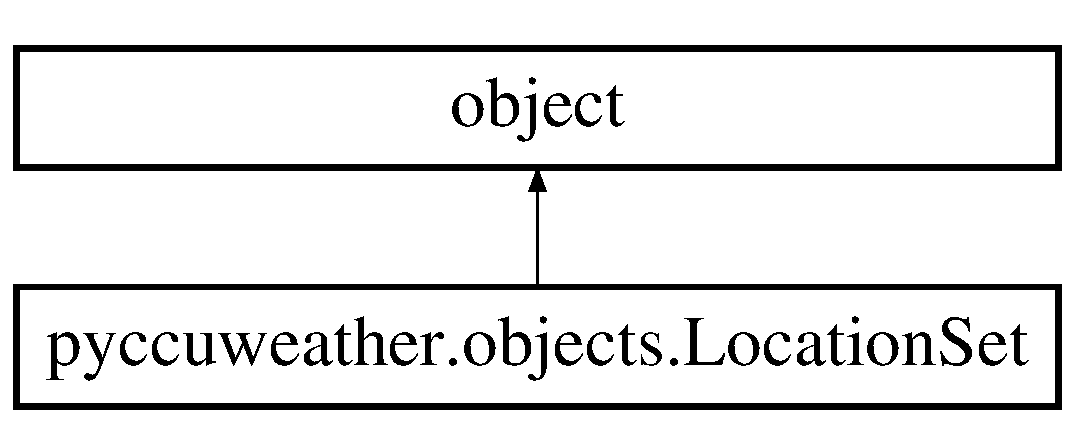
\includegraphics[height=2.000000cm]{classpyccuweather_1_1objects_1_1_location_set}
\end{center}
\end{figure}
\subsection*{Public Member Functions}
\begin{DoxyCompactItemize}
\item 
\hypertarget{classpyccuweather_1_1objects_1_1_location_set_af51b3500bda3b16d0930ec86a79b76c8}{}def {\bfseries \+\_\+\+\_\+init\+\_\+\+\_\+}\label{classpyccuweather_1_1objects_1_1_location_set_af51b3500bda3b16d0930ec86a79b76c8}

\item 
\hypertarget{classpyccuweather_1_1objects_1_1_location_set_a189b48a13f608d5acb391159c5416786}{}def {\bfseries \+\_\+\+\_\+len\+\_\+\+\_\+} (self)\label{classpyccuweather_1_1objects_1_1_location_set_a189b48a13f608d5acb391159c5416786}

\item 
\hypertarget{classpyccuweather_1_1objects_1_1_location_set_a947c16f6d0d87712c1a86dc403bb061c}{}def {\bfseries \+\_\+\+\_\+getitem\+\_\+\+\_\+} (self, item)\label{classpyccuweather_1_1objects_1_1_location_set_a947c16f6d0d87712c1a86dc403bb061c}

\item 
\hypertarget{classpyccuweather_1_1objects_1_1_location_set_a77d97f02ed7d3848ad69dbe73316498e}{}def {\bfseries \+\_\+\+\_\+str\+\_\+\+\_\+} (self)\label{classpyccuweather_1_1objects_1_1_location_set_a77d97f02ed7d3848ad69dbe73316498e}

\item 
\hypertarget{classpyccuweather_1_1objects_1_1_location_set_a23452d99d69522931f6f9fa542ad200e}{}def {\bfseries append}\label{classpyccuweather_1_1objects_1_1_location_set_a23452d99d69522931f6f9fa542ad200e}

\end{DoxyCompactItemize}
\subsection*{Public Attributes}
\begin{DoxyCompactItemize}
\item 
\hypertarget{classpyccuweather_1_1objects_1_1_location_set_a5f63f2f977086d7c01d2c0f51eb6f4d0}{}{\bfseries results}\label{classpyccuweather_1_1objects_1_1_location_set_a5f63f2f977086d7c01d2c0f51eb6f4d0}

\item 
\hypertarget{classpyccuweather_1_1objects_1_1_location_set_a364247fec86f6ce933fc477e1058ba98}{}{\bfseries search\+\_\+expression}\label{classpyccuweather_1_1objects_1_1_location_set_a364247fec86f6ce933fc477e1058ba98}

\item 
\hypertarget{classpyccuweather_1_1objects_1_1_location_set_ab2e81d7a058dd87a8cbce8fcaae63317}{}{\bfseries country}\label{classpyccuweather_1_1objects_1_1_location_set_ab2e81d7a058dd87a8cbce8fcaae63317}

\end{DoxyCompactItemize}


\subsection{Detailed Description}
\begin{DoxyVerb}Represents a set of Locations returned usually as a search result.
\end{DoxyVerb}
 

The documentation for this class was generated from the following file\+:\begin{DoxyCompactItemize}
\item 
pyccuweather/objects.\+py\end{DoxyCompactItemize}

\hypertarget{classpyccuweather_1_1errors_1_1_malformatted_a_p_i_key_error}{}\section{pyccuweather.\+errors.\+Malformatted\+A\+P\+I\+Key\+Error Class Reference}
\label{classpyccuweather_1_1errors_1_1_malformatted_a_p_i_key_error}\index{pyccuweather.\+errors.\+Malformatted\+A\+P\+I\+Key\+Error@{pyccuweather.\+errors.\+Malformatted\+A\+P\+I\+Key\+Error}}
Inheritance diagram for pyccuweather.\+errors.\+Malformatted\+A\+P\+I\+Key\+Error\+:\begin{figure}[H]
\begin{center}
\leavevmode
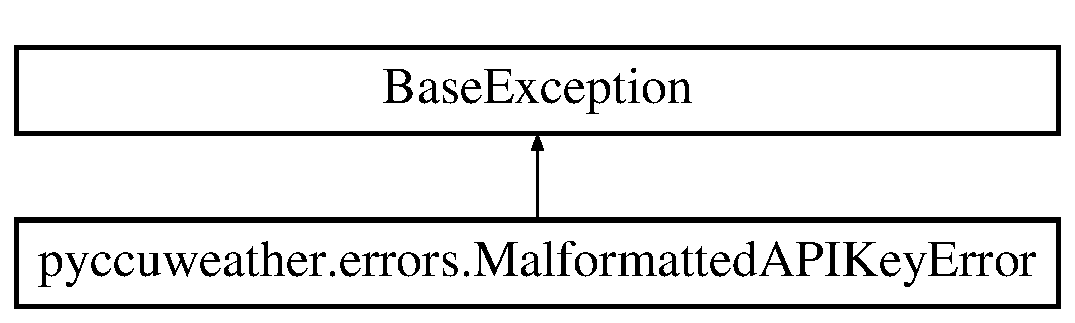
\includegraphics[height=2.000000cm]{classpyccuweather_1_1errors_1_1_malformatted_a_p_i_key_error}
\end{center}
\end{figure}
\subsection*{Public Member Functions}
\begin{DoxyCompactItemize}
\item 
\hypertarget{classpyccuweather_1_1errors_1_1_malformatted_a_p_i_key_error_a1820a7856806a94b1dceae84bb00f8fd}{}def {\bfseries \+\_\+\+\_\+str\+\_\+\+\_\+} (self)\label{classpyccuweather_1_1errors_1_1_malformatted_a_p_i_key_error_a1820a7856806a94b1dceae84bb00f8fd}

\end{DoxyCompactItemize}


\subsection{Detailed Description}
\begin{DoxyVerb}Raised when the API key looks malformatted (wrong type or length). Does not actually check the API key for validity!"
\end{DoxyVerb}
 

The documentation for this class was generated from the following file\+:\begin{DoxyCompactItemize}
\item 
pyccuweather/errors.\+py\end{DoxyCompactItemize}

\hypertarget{classpyccuweather_1_1errors_1_1_malformatted_location_key_error}{}\section{pyccuweather.\+errors.\+Malformatted\+Location\+Key\+Error Class Reference}
\label{classpyccuweather_1_1errors_1_1_malformatted_location_key_error}\index{pyccuweather.\+errors.\+Malformatted\+Location\+Key\+Error@{pyccuweather.\+errors.\+Malformatted\+Location\+Key\+Error}}
Inheritance diagram for pyccuweather.\+errors.\+Malformatted\+Location\+Key\+Error\+:\begin{figure}[H]
\begin{center}
\leavevmode
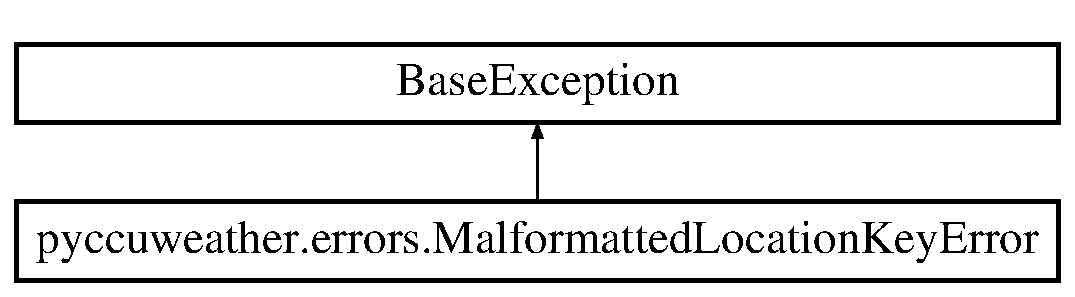
\includegraphics[height=2.000000cm]{classpyccuweather_1_1errors_1_1_malformatted_location_key_error}
\end{center}
\end{figure}
\subsection*{Public Member Functions}
\begin{DoxyCompactItemize}
\item 
\hypertarget{classpyccuweather_1_1errors_1_1_malformatted_location_key_error_a4f66007a86cecc6fcd3273f9e6947ad4}{}def {\bfseries \+\_\+\+\_\+str\+\_\+\+\_\+} (self)\label{classpyccuweather_1_1errors_1_1_malformatted_location_key_error_a4f66007a86cecc6fcd3273f9e6947ad4}

\end{DoxyCompactItemize}


\subsection{Detailed Description}
\begin{DoxyVerb}The location key is malformatted. This is raised when a primary (non-POI) location key is entered that does not fit
the formal specifications.
\end{DoxyVerb}
 

The documentation for this class was generated from the following file\+:\begin{DoxyCompactItemize}
\item 
pyccuweather/errors.\+py\end{DoxyCompactItemize}

\hypertarget{classpyccuweather_1_1errors_1_1_no_location_error}{}\section{pyccuweather.\+errors.\+No\+Location\+Error Class Reference}
\label{classpyccuweather_1_1errors_1_1_no_location_error}\index{pyccuweather.\+errors.\+No\+Location\+Error@{pyccuweather.\+errors.\+No\+Location\+Error}}
Inheritance diagram for pyccuweather.\+errors.\+No\+Location\+Error\+:\begin{figure}[H]
\begin{center}
\leavevmode
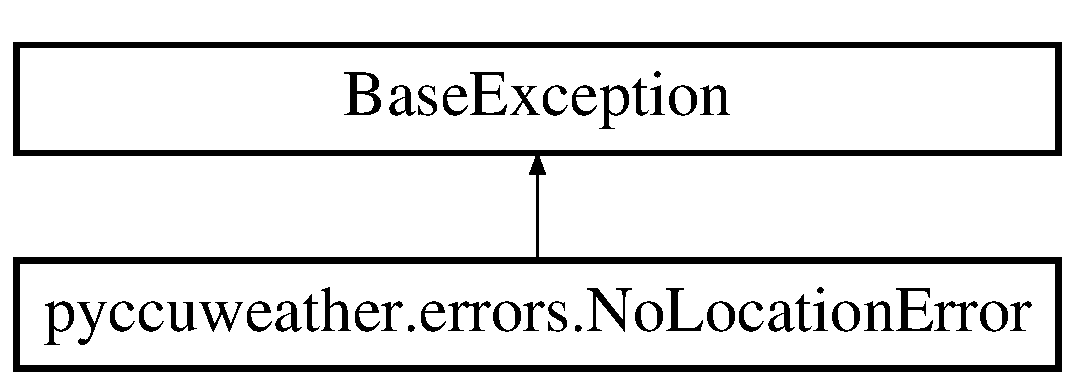
\includegraphics[height=2.000000cm]{classpyccuweather_1_1errors_1_1_no_location_error}
\end{center}
\end{figure}
\subsection*{Public Member Functions}
\begin{DoxyCompactItemize}
\item 
\hypertarget{classpyccuweather_1_1errors_1_1_no_location_error_a85c98a0aa027190c5b7ec7100565f8e5}{}def {\bfseries \+\_\+\+\_\+init\+\_\+\+\_\+} (self, lat, lon)\label{classpyccuweather_1_1errors_1_1_no_location_error_a85c98a0aa027190c5b7ec7100565f8e5}

\item 
\hypertarget{classpyccuweather_1_1errors_1_1_no_location_error_adbfbbfb0c27f22f536c0bd2cf1e8a9a0}{}def {\bfseries \+\_\+\+\_\+str\+\_\+\+\_\+} (self)\label{classpyccuweather_1_1errors_1_1_no_location_error_adbfbbfb0c27f22f536c0bd2cf1e8a9a0}

\end{DoxyCompactItemize}
\subsection*{Public Attributes}
\begin{DoxyCompactItemize}
\item 
\hypertarget{classpyccuweather_1_1errors_1_1_no_location_error_a62c196dbabf819f8ac23d9219091f64c}{}{\bfseries lat}\label{classpyccuweather_1_1errors_1_1_no_location_error_a62c196dbabf819f8ac23d9219091f64c}

\item 
\hypertarget{classpyccuweather_1_1errors_1_1_no_location_error_a4ebcd15e499e59fa5f691d55aa4845fa}{}{\bfseries lon}\label{classpyccuweather_1_1errors_1_1_no_location_error_a4ebcd15e499e59fa5f691d55aa4845fa}

\end{DoxyCompactItemize}


\subsection{Detailed Description}
\begin{DoxyVerb}Raised when the coordinates do not resolve to a particular location.
\end{DoxyVerb}
 

The documentation for this class was generated from the following file\+:\begin{DoxyCompactItemize}
\item 
pyccuweather/errors.\+py\end{DoxyCompactItemize}

\hypertarget{classpyccuweather_1_1errors_1_1_no_results_error}{}\section{pyccuweather.\+errors.\+No\+Results\+Error Class Reference}
\label{classpyccuweather_1_1errors_1_1_no_results_error}\index{pyccuweather.\+errors.\+No\+Results\+Error@{pyccuweather.\+errors.\+No\+Results\+Error}}
Inheritance diagram for pyccuweather.\+errors.\+No\+Results\+Error\+:\begin{figure}[H]
\begin{center}
\leavevmode
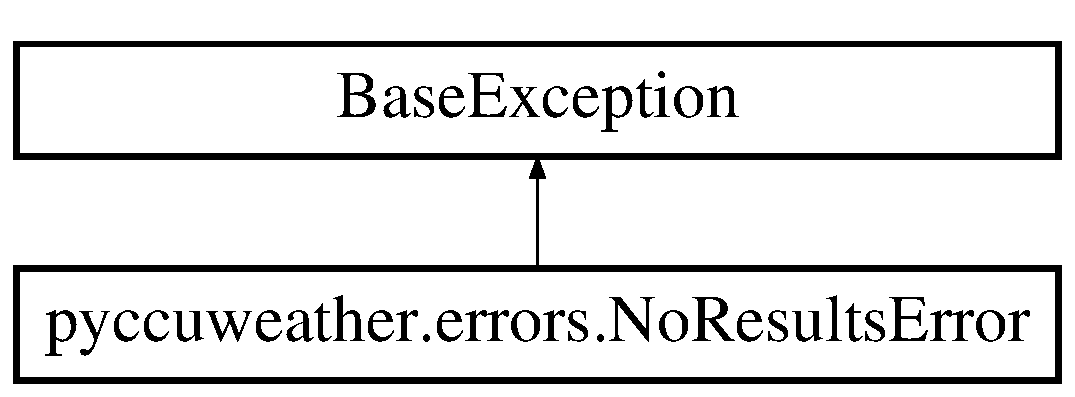
\includegraphics[height=2.000000cm]{classpyccuweather_1_1errors_1_1_no_results_error}
\end{center}
\end{figure}
\subsection*{Public Member Functions}
\begin{DoxyCompactItemize}
\item 
\hypertarget{classpyccuweather_1_1errors_1_1_no_results_error_ab671979f5d4914e2b20f942161b1d1fc}{}def {\bfseries \+\_\+\+\_\+init\+\_\+\+\_\+} (self, query)\label{classpyccuweather_1_1errors_1_1_no_results_error_ab671979f5d4914e2b20f942161b1d1fc}

\item 
\hypertarget{classpyccuweather_1_1errors_1_1_no_results_error_addf01ff5fb6de6e7adbea60c3591b5a0}{}def {\bfseries \+\_\+\+\_\+str\+\_\+\+\_\+} (self)\label{classpyccuweather_1_1errors_1_1_no_results_error_addf01ff5fb6de6e7adbea60c3591b5a0}

\end{DoxyCompactItemize}
\subsection*{Public Attributes}
\begin{DoxyCompactItemize}
\item 
\hypertarget{classpyccuweather_1_1errors_1_1_no_results_error_a97d7016ae414702e5ce3b28e69ae48ed}{}{\bfseries query}\label{classpyccuweather_1_1errors_1_1_no_results_error_a97d7016ae414702e5ce3b28e69ae48ed}

\end{DoxyCompactItemize}


\subsection{Detailed Description}
\begin{DoxyVerb}Yielded when a query has no results.
\end{DoxyVerb}
 

The documentation for this class was generated from the following file\+:\begin{DoxyCompactItemize}
\item 
pyccuweather/errors.\+py\end{DoxyCompactItemize}

\hypertarget{classpyccuweather_1_1errors_1_1_not_implemented_or_unknown_method}{}\section{pyccuweather.\+errors.\+Not\+Implemented\+Or\+Unknown\+Method Class Reference}
\label{classpyccuweather_1_1errors_1_1_not_implemented_or_unknown_method}\index{pyccuweather.\+errors.\+Not\+Implemented\+Or\+Unknown\+Method@{pyccuweather.\+errors.\+Not\+Implemented\+Or\+Unknown\+Method}}
Inheritance diagram for pyccuweather.\+errors.\+Not\+Implemented\+Or\+Unknown\+Method\+:\begin{figure}[H]
\begin{center}
\leavevmode
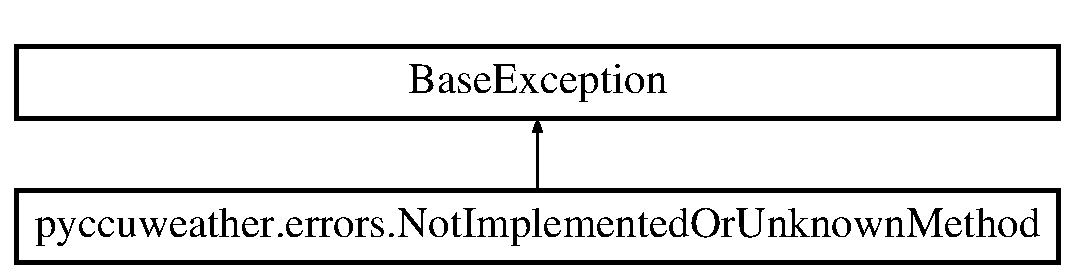
\includegraphics[height=2.000000cm]{classpyccuweather_1_1errors_1_1_not_implemented_or_unknown_method}
\end{center}
\end{figure}
\subsection*{Public Member Functions}
\begin{DoxyCompactItemize}
\item 
\hypertarget{classpyccuweather_1_1errors_1_1_not_implemented_or_unknown_method_a7528d7704d9365a1b4a3a237d845cc0f}{}def {\bfseries \+\_\+\+\_\+init\+\_\+\+\_\+} (self, A\+P\+I\+\_\+method)\label{classpyccuweather_1_1errors_1_1_not_implemented_or_unknown_method_a7528d7704d9365a1b4a3a237d845cc0f}

\item 
\hypertarget{classpyccuweather_1_1errors_1_1_not_implemented_or_unknown_method_a915ece839cebfbb92f9b0ff1084ebb61}{}def {\bfseries \+\_\+\+\_\+str\+\_\+\+\_\+} (self)\label{classpyccuweather_1_1errors_1_1_not_implemented_or_unknown_method_a915ece839cebfbb92f9b0ff1084ebb61}

\end{DoxyCompactItemize}
\subsection*{Public Attributes}
\begin{DoxyCompactItemize}
\item 
\hypertarget{classpyccuweather_1_1errors_1_1_not_implemented_or_unknown_method_a3e66e277e85cb9815c13ed91da4210e9}{}{\bfseries A\+P\+I\+\_\+method}\label{classpyccuweather_1_1errors_1_1_not_implemented_or_unknown_method_a3e66e277e85cb9815c13ed91da4210e9}

\end{DoxyCompactItemize}


\subsection{Detailed Description}
\begin{DoxyVerb}The method called has not been implemented yet or is an altogether non-existent method.
\end{DoxyVerb}
 

The documentation for this class was generated from the following file\+:\begin{DoxyCompactItemize}
\item 
pyccuweather/errors.\+py\end{DoxyCompactItemize}

\hypertarget{classpyccuweather_1_1objects_1_1_observation}{}\section{pyccuweather.\+objects.\+Observation Class Reference}
\label{classpyccuweather_1_1objects_1_1_observation}\index{pyccuweather.\+objects.\+Observation@{pyccuweather.\+objects.\+Observation}}
Inheritance diagram for pyccuweather.\+objects.\+Observation\+:\begin{figure}[H]
\begin{center}
\leavevmode
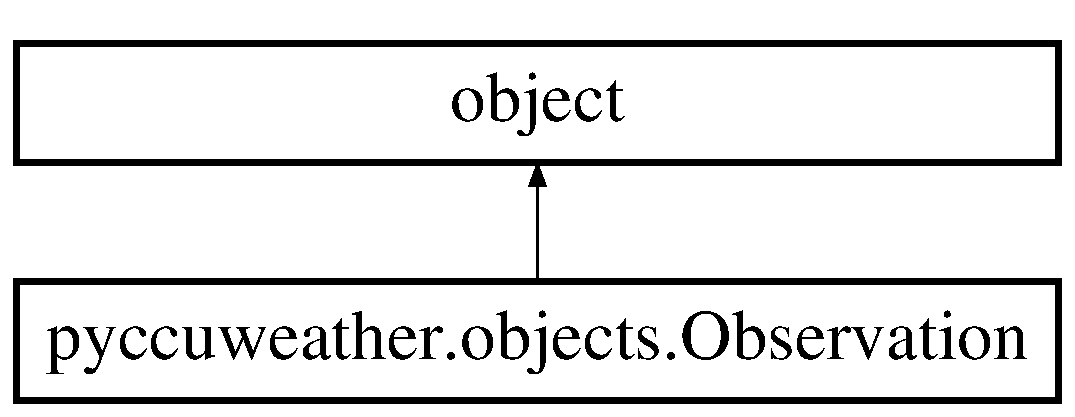
\includegraphics[height=2.000000cm]{classpyccuweather_1_1objects_1_1_observation}
\end{center}
\end{figure}
\subsection*{Public Member Functions}
\begin{DoxyCompactItemize}
\item 
\hypertarget{classpyccuweather_1_1objects_1_1_observation_a319e70e2c445a5109fb3709768263dfa}{}def {\bfseries \+\_\+\+\_\+init\+\_\+\+\_\+} (self, json)\label{classpyccuweather_1_1objects_1_1_observation_a319e70e2c445a5109fb3709768263dfa}

\item 
\hypertarget{classpyccuweather_1_1objects_1_1_observation_ab9fb3d1f9a1812c3a0f7cd063f72015c}{}def {\bfseries \+\_\+\+\_\+str\+\_\+\+\_\+} (self)\label{classpyccuweather_1_1objects_1_1_observation_ab9fb3d1f9a1812c3a0f7cd063f72015c}

\end{DoxyCompactItemize}
\subsection*{Public Attributes}
\begin{DoxyCompactItemize}
\item 
\hypertarget{classpyccuweather_1_1objects_1_1_observation_a362b6721e246f2717a7e8e3919fbf69a}{}{\bfseries date\+\_\+time}\label{classpyccuweather_1_1objects_1_1_observation_a362b6721e246f2717a7e8e3919fbf69a}

\item 
\hypertarget{classpyccuweather_1_1objects_1_1_observation_af669838251f2ce9fb212eb1a09c23094}{}{\bfseries epoch\+\_\+time}\label{classpyccuweather_1_1objects_1_1_observation_af669838251f2ce9fb212eb1a09c23094}

\item 
\hypertarget{classpyccuweather_1_1objects_1_1_observation_aa311068344ac25e4788bc5c8e68d2f14}{}{\bfseries synopsis}\label{classpyccuweather_1_1objects_1_1_observation_aa311068344ac25e4788bc5c8e68d2f14}

\item 
\hypertarget{classpyccuweather_1_1objects_1_1_observation_ad6c6b3bdf1c2b9d224f3d7478f57bc02}{}{\bfseries temperature}\label{classpyccuweather_1_1objects_1_1_observation_ad6c6b3bdf1c2b9d224f3d7478f57bc02}

\item 
\hypertarget{classpyccuweather_1_1objects_1_1_observation_a7a35bdfb9d10219d70fbdea32d732be5}{}{\bfseries link}\label{classpyccuweather_1_1objects_1_1_observation_a7a35bdfb9d10219d70fbdea32d732be5}

\item 
\hypertarget{classpyccuweather_1_1objects_1_1_observation_a7f66f75b110a011e1bb71856292a1056}{}{\bfseries mobile\+\_\+link}\label{classpyccuweather_1_1objects_1_1_observation_a7f66f75b110a011e1bb71856292a1056}

\item 
\hypertarget{classpyccuweather_1_1objects_1_1_observation_a74a072536980091fdf545c6c013d30f1}{}{\bfseries raw}\label{classpyccuweather_1_1objects_1_1_observation_a74a072536980091fdf545c6c013d30f1}

\end{DoxyCompactItemize}


The documentation for this class was generated from the following file\+:\begin{DoxyCompactItemize}
\item 
pyccuweather/objects.\+py\end{DoxyCompactItemize}

\hypertarget{classpyccuweather_1_1objects_1_1_precipitation}{}\section{pyccuweather.\+objects.\+Precipitation Class Reference}
\label{classpyccuweather_1_1objects_1_1_precipitation}\index{pyccuweather.\+objects.\+Precipitation@{pyccuweather.\+objects.\+Precipitation}}
Inheritance diagram for pyccuweather.\+objects.\+Precipitation\+:\begin{figure}[H]
\begin{center}
\leavevmode
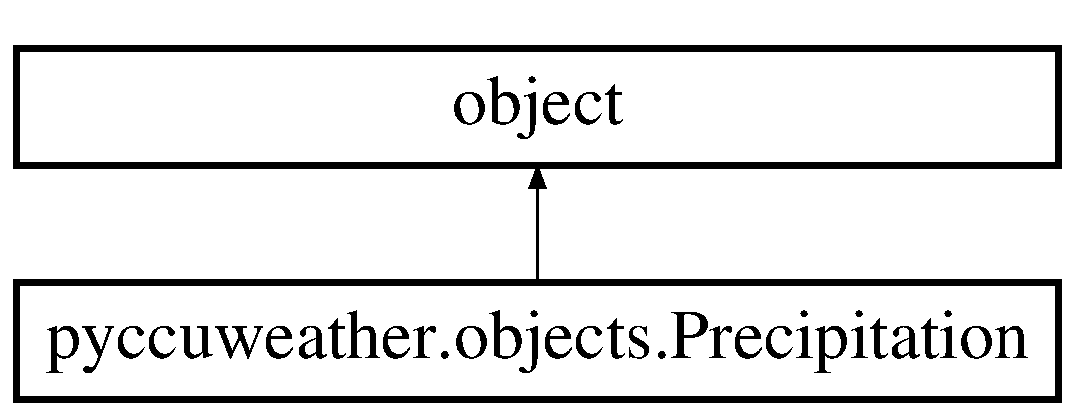
\includegraphics[height=2.000000cm]{classpyccuweather_1_1objects_1_1_precipitation}
\end{center}
\end{figure}
\subsection*{Public Member Functions}
\begin{DoxyCompactItemize}
\item 
\hypertarget{classpyccuweather_1_1objects_1_1_precipitation_a5ffbf00c9b8eacdbcba345c1fbbfabf2}{}def {\bfseries \+\_\+\+\_\+init\+\_\+\+\_\+}\label{classpyccuweather_1_1objects_1_1_precipitation_a5ffbf00c9b8eacdbcba345c1fbbfabf2}

\item 
def \hyperlink{classpyccuweather_1_1objects_1_1_precipitation_a581b3112ef01ae6556ca8e4c204e2115}{mm} (self)
\item 
def \hyperlink{classpyccuweather_1_1objects_1_1_precipitation_a3307c99c0b042d504cdbe1431f0d4251}{inch} (self)
\item 
\hypertarget{classpyccuweather_1_1objects_1_1_precipitation_ae880fb9914853a7cbc3bb155bcc48dc8}{}def {\bfseries \+\_\+\+\_\+str\+\_\+\+\_\+} (self)\label{classpyccuweather_1_1objects_1_1_precipitation_ae880fb9914853a7cbc3bb155bcc48dc8}

\end{DoxyCompactItemize}
\subsection*{Public Attributes}
\begin{DoxyCompactItemize}
\item 
\hypertarget{classpyccuweather_1_1objects_1_1_precipitation_a04d15b0c527ceb6f82f4f686e1bc6b49}{}{\bfseries value}\label{classpyccuweather_1_1objects_1_1_precipitation_a04d15b0c527ceb6f82f4f686e1bc6b49}

\item 
\hypertarget{classpyccuweather_1_1objects_1_1_precipitation_a86d6ad010715eccd5a2c7161e7b3bbd1}{}{\bfseries units}\label{classpyccuweather_1_1objects_1_1_precipitation_a86d6ad010715eccd5a2c7161e7b3bbd1}

\end{DoxyCompactItemize}


\subsection{Detailed Description}
\begin{DoxyVerb}Represents a precipitation value.
\end{DoxyVerb}
 

\subsection{Member Function Documentation}
\hypertarget{classpyccuweather_1_1objects_1_1_precipitation_a3307c99c0b042d504cdbe1431f0d4251}{}\index{pyccuweather\+::objects\+::\+Precipitation@{pyccuweather\+::objects\+::\+Precipitation}!inch@{inch}}
\index{inch@{inch}!pyccuweather\+::objects\+::\+Precipitation@{pyccuweather\+::objects\+::\+Precipitation}}
\subsubsection[{inch}]{\setlength{\rightskip}{0pt plus 5cm}def pyccuweather.\+objects.\+Precipitation.\+inch (
\begin{DoxyParamCaption}
\item[{}]{self}
\end{DoxyParamCaption}
)}\label{classpyccuweather_1_1objects_1_1_precipitation_a3307c99c0b042d504cdbe1431f0d4251}
\begin{DoxyVerb}Represents precipitation in inches.

:return: precipitation in in
\end{DoxyVerb}
 \hypertarget{classpyccuweather_1_1objects_1_1_precipitation_a581b3112ef01ae6556ca8e4c204e2115}{}\index{pyccuweather\+::objects\+::\+Precipitation@{pyccuweather\+::objects\+::\+Precipitation}!mm@{mm}}
\index{mm@{mm}!pyccuweather\+::objects\+::\+Precipitation@{pyccuweather\+::objects\+::\+Precipitation}}
\subsubsection[{mm}]{\setlength{\rightskip}{0pt plus 5cm}def pyccuweather.\+objects.\+Precipitation.\+mm (
\begin{DoxyParamCaption}
\item[{}]{self}
\end{DoxyParamCaption}
)}\label{classpyccuweather_1_1objects_1_1_precipitation_a581b3112ef01ae6556ca8e4c204e2115}
\begin{DoxyVerb}Represents precipitation in mm.

:return: precipitation in mm
\end{DoxyVerb}
 

The documentation for this class was generated from the following file\+:\begin{DoxyCompactItemize}
\item 
pyccuweather/objects.\+py\end{DoxyCompactItemize}

\hypertarget{classpyccuweather_1_1errors_1_1_range_error}{}\section{pyccuweather.\+errors.\+Range\+Error Class Reference}
\label{classpyccuweather_1_1errors_1_1_range_error}\index{pyccuweather.\+errors.\+Range\+Error@{pyccuweather.\+errors.\+Range\+Error}}
Inheritance diagram for pyccuweather.\+errors.\+Range\+Error\+:\begin{figure}[H]
\begin{center}
\leavevmode
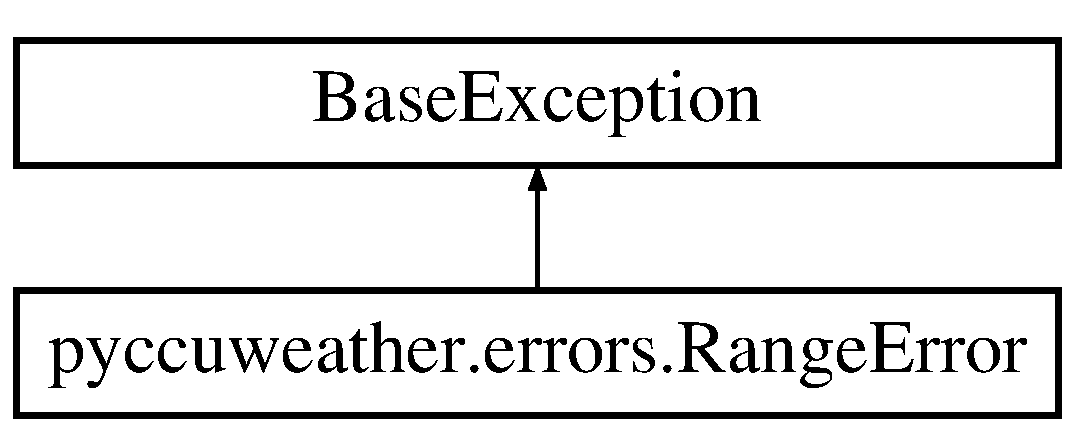
\includegraphics[height=2.000000cm]{classpyccuweather_1_1errors_1_1_range_error}
\end{center}
\end{figure}
\subsection*{Public Member Functions}
\begin{DoxyCompactItemize}
\item 
\hypertarget{classpyccuweather_1_1errors_1_1_range_error_ad82eb8a20cdd96338a8f0cf4263439da}{}def {\bfseries \+\_\+\+\_\+str\+\_\+\+\_\+} (self)\label{classpyccuweather_1_1errors_1_1_range_error_ad82eb8a20cdd96338a8f0cf4263439da}

\end{DoxyCompactItemize}


\subsection{Detailed Description}
\begin{DoxyVerb}Raised when the coordinates provided are out of range.
\end{DoxyVerb}
 

The documentation for this class was generated from the following file\+:\begin{DoxyCompactItemize}
\item 
pyccuweather/errors.\+py\end{DoxyCompactItemize}

\hypertarget{classpyccuweather_1_1objects_1_1_region}{}\section{pyccuweather.\+objects.\+Region Class Reference}
\label{classpyccuweather_1_1objects_1_1_region}\index{pyccuweather.\+objects.\+Region@{pyccuweather.\+objects.\+Region}}
Inheritance diagram for pyccuweather.\+objects.\+Region\+:\begin{figure}[H]
\begin{center}
\leavevmode
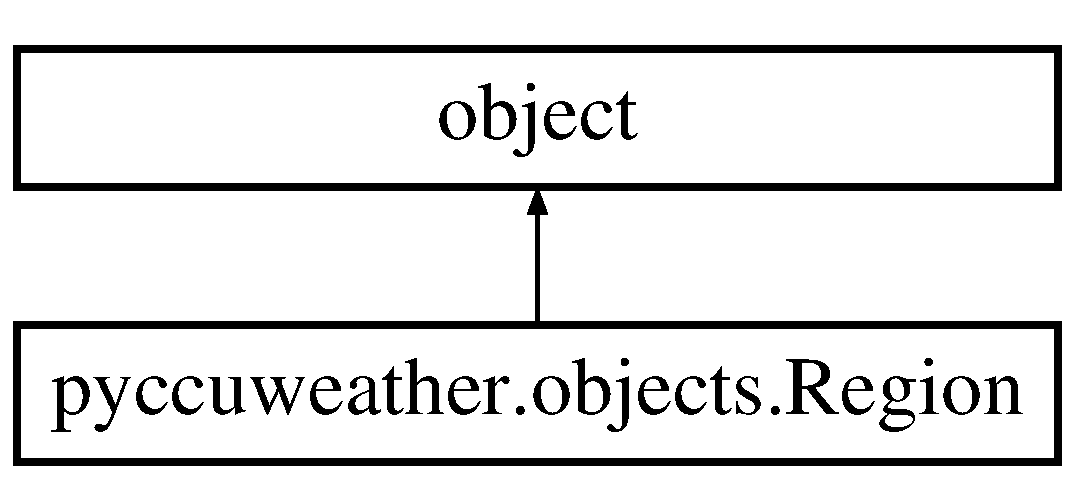
\includegraphics[height=2.000000cm]{classpyccuweather_1_1objects_1_1_region}
\end{center}
\end{figure}
\subsection*{Public Member Functions}
\begin{DoxyCompactItemize}
\item 
\hypertarget{classpyccuweather_1_1objects_1_1_region_a6e0c994649920851d4b7663c84e925e9}{}def {\bfseries \+\_\+\+\_\+init\+\_\+\+\_\+}\label{classpyccuweather_1_1objects_1_1_region_a6e0c994649920851d4b7663c84e925e9}

\item 
\hypertarget{classpyccuweather_1_1objects_1_1_region_a0288fc9bc476e70a1554bd78c72f9709}{}def {\bfseries \+\_\+\+\_\+str\+\_\+\+\_\+} (self)\label{classpyccuweather_1_1objects_1_1_region_a0288fc9bc476e70a1554bd78c72f9709}

\end{DoxyCompactItemize}
\subsection*{Public Attributes}
\begin{DoxyCompactItemize}
\item 
\hypertarget{classpyccuweather_1_1objects_1_1_region_a8b22e132f3f4f11e45dc53a2e4651b91}{}{\bfseries id}\label{classpyccuweather_1_1objects_1_1_region_a8b22e132f3f4f11e45dc53a2e4651b91}

\item 
\hypertarget{classpyccuweather_1_1objects_1_1_region_a92b68f1cabb88148305003393def659c}{}{\bfseries localized\+\_\+name}\label{classpyccuweather_1_1objects_1_1_region_a92b68f1cabb88148305003393def659c}

\item 
\hypertarget{classpyccuweather_1_1objects_1_1_region_a6fbfd568b12248b7594b721b4546f7b9}{}{\bfseries english\+\_\+name}\label{classpyccuweather_1_1objects_1_1_region_a6fbfd568b12248b7594b721b4546f7b9}

\end{DoxyCompactItemize}


\subsection{Detailed Description}
\begin{DoxyVerb}An object representing an Accuweather Region.
For a list of Accuweather regions: http://apidev.accuweather.com/developers/regions
\end{DoxyVerb}
 

The documentation for this class was generated from the following file\+:\begin{DoxyCompactItemize}
\item 
pyccuweather/objects.\+py\end{DoxyCompactItemize}

\hypertarget{classpyccuweather_1_1objects_1_1_snow}{}\section{pyccuweather.\+objects.\+Snow Class Reference}
\label{classpyccuweather_1_1objects_1_1_snow}\index{pyccuweather.\+objects.\+Snow@{pyccuweather.\+objects.\+Snow}}
Inheritance diagram for pyccuweather.\+objects.\+Snow\+:\begin{figure}[H]
\begin{center}
\leavevmode
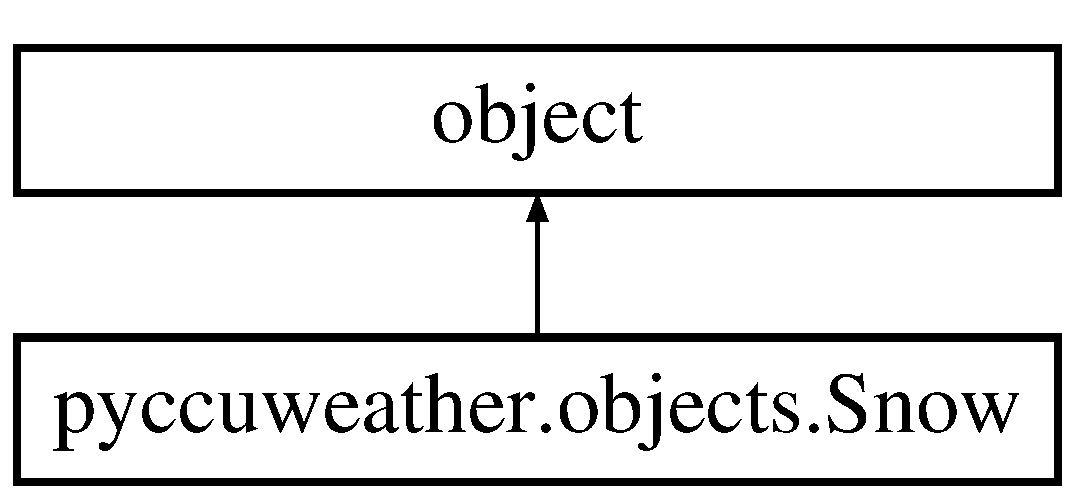
\includegraphics[height=2.000000cm]{classpyccuweather_1_1objects_1_1_snow}
\end{center}
\end{figure}
\subsection*{Public Member Functions}
\begin{DoxyCompactItemize}
\item 
\hypertarget{classpyccuweather_1_1objects_1_1_snow_ae0848ebe5fd948badf776a7dccb52fa6}{}def {\bfseries \+\_\+\+\_\+init\+\_\+\+\_\+}\label{classpyccuweather_1_1objects_1_1_snow_ae0848ebe5fd948badf776a7dccb52fa6}

\item 
\hypertarget{classpyccuweather_1_1objects_1_1_snow_a9d6ae3ea75aee9a8c5cd49e562159161}{}def {\bfseries mm} (self)\label{classpyccuweather_1_1objects_1_1_snow_a9d6ae3ea75aee9a8c5cd49e562159161}

\item 
\hypertarget{classpyccuweather_1_1objects_1_1_snow_af18371e5934d596bb02763b76e197b63}{}def {\bfseries inch} (self)\label{classpyccuweather_1_1objects_1_1_snow_af18371e5934d596bb02763b76e197b63}

\item 
\hypertarget{classpyccuweather_1_1objects_1_1_snow_a70d3f82377ec3fac366ee9bfc3418a33}{}def {\bfseries \+\_\+\+\_\+str\+\_\+\+\_\+} (self)\label{classpyccuweather_1_1objects_1_1_snow_a70d3f82377ec3fac366ee9bfc3418a33}

\end{DoxyCompactItemize}
\subsection*{Public Attributes}
\begin{DoxyCompactItemize}
\item 
\hypertarget{classpyccuweather_1_1objects_1_1_snow_adf35f750b34db23f908129bbdef4dc3b}{}{\bfseries value}\label{classpyccuweather_1_1objects_1_1_snow_adf35f750b34db23f908129bbdef4dc3b}

\item 
\hypertarget{classpyccuweather_1_1objects_1_1_snow_a41d2a5ab15c5d60b1e586b0e25b3d040}{}{\bfseries units}\label{classpyccuweather_1_1objects_1_1_snow_a41d2a5ab15c5d60b1e586b0e25b3d040}

\end{DoxyCompactItemize}


The documentation for this class was generated from the following file\+:\begin{DoxyCompactItemize}
\item 
pyccuweather/objects.\+py\end{DoxyCompactItemize}

\hypertarget{classpyccuweather_1_1objects_1_1_temperature}{}\section{pyccuweather.\+objects.\+Temperature Class Reference}
\label{classpyccuweather_1_1objects_1_1_temperature}\index{pyccuweather.\+objects.\+Temperature@{pyccuweather.\+objects.\+Temperature}}
Inheritance diagram for pyccuweather.\+objects.\+Temperature\+:\begin{figure}[H]
\begin{center}
\leavevmode
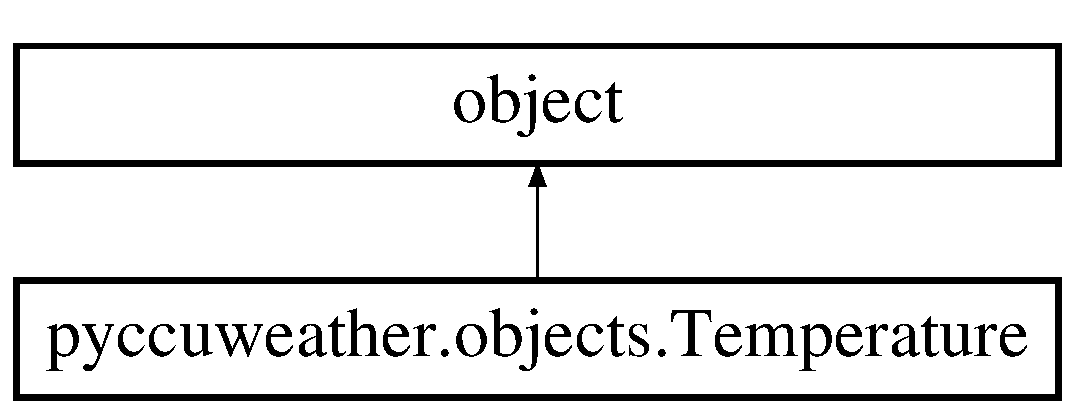
\includegraphics[height=2.000000cm]{classpyccuweather_1_1objects_1_1_temperature}
\end{center}
\end{figure}
\subsection*{Public Member Functions}
\begin{DoxyCompactItemize}
\item 
\hypertarget{classpyccuweather_1_1objects_1_1_temperature_a0b6c5c7abaa9244806b7fa16b3d4e9f3}{}def {\bfseries \+\_\+\+\_\+init\+\_\+\+\_\+}\label{classpyccuweather_1_1objects_1_1_temperature_a0b6c5c7abaa9244806b7fa16b3d4e9f3}

\item 
def \hyperlink{classpyccuweather_1_1objects_1_1_temperature_a6331f9e12224775c19c27eec5f26a3c7}{F} (self)
\item 
def \hyperlink{classpyccuweather_1_1objects_1_1_temperature_a4b1adae2885e87eceff3127af1b46a3c}{C} (self)
\item 
\hypertarget{classpyccuweather_1_1objects_1_1_temperature_a1ec2241a99c0030a9a70199e6b2da037}{}def {\bfseries \+\_\+\+\_\+str\+\_\+\+\_\+} (self)\label{classpyccuweather_1_1objects_1_1_temperature_a1ec2241a99c0030a9a70199e6b2da037}

\end{DoxyCompactItemize}
\subsection*{Public Attributes}
\begin{DoxyCompactItemize}
\item 
\hypertarget{classpyccuweather_1_1objects_1_1_temperature_ac54036fc8d9d545dc8c153dec17eeacb}{}{\bfseries value}\label{classpyccuweather_1_1objects_1_1_temperature_ac54036fc8d9d545dc8c153dec17eeacb}

\item 
\hypertarget{classpyccuweather_1_1objects_1_1_temperature_ac6cd3e7f652318fc3b3c84ffec313756}{}{\bfseries units}\label{classpyccuweather_1_1objects_1_1_temperature_ac6cd3e7f652318fc3b3c84ffec313756}

\end{DoxyCompactItemize}


\subsection{Detailed Description}
\begin{DoxyVerb}Represents a temperature value.
\end{DoxyVerb}
 

\subsection{Member Function Documentation}
\hypertarget{classpyccuweather_1_1objects_1_1_temperature_a4b1adae2885e87eceff3127af1b46a3c}{}\index{pyccuweather\+::objects\+::\+Temperature@{pyccuweather\+::objects\+::\+Temperature}!C@{C}}
\index{C@{C}!pyccuweather\+::objects\+::\+Temperature@{pyccuweather\+::objects\+::\+Temperature}}
\subsubsection[{C}]{\setlength{\rightskip}{0pt plus 5cm}def pyccuweather.\+objects.\+Temperature.\+C (
\begin{DoxyParamCaption}
\item[{}]{self}
\end{DoxyParamCaption}
)}\label{classpyccuweather_1_1objects_1_1_temperature_a4b1adae2885e87eceff3127af1b46a3c}
\begin{DoxyVerb}Represents the Temperature in Celsius.

:return: Temperature in degrees Celsius.
\end{DoxyVerb}
 \hypertarget{classpyccuweather_1_1objects_1_1_temperature_a6331f9e12224775c19c27eec5f26a3c7}{}\index{pyccuweather\+::objects\+::\+Temperature@{pyccuweather\+::objects\+::\+Temperature}!F@{F}}
\index{F@{F}!pyccuweather\+::objects\+::\+Temperature@{pyccuweather\+::objects\+::\+Temperature}}
\subsubsection[{F}]{\setlength{\rightskip}{0pt plus 5cm}def pyccuweather.\+objects.\+Temperature.\+F (
\begin{DoxyParamCaption}
\item[{}]{self}
\end{DoxyParamCaption}
)}\label{classpyccuweather_1_1objects_1_1_temperature_a6331f9e12224775c19c27eec5f26a3c7}
\begin{DoxyVerb}Represents the Temperature in Fahrenheit.

:return: Temperature in degrees Fahrenheit.
\end{DoxyVerb}
 

The documentation for this class was generated from the following file\+:\begin{DoxyCompactItemize}
\item 
pyccuweather/objects.\+py\end{DoxyCompactItemize}

\hypertarget{classpyccuweather_1_1objects_1_1_time_zone}{}\section{pyccuweather.\+objects.\+Time\+Zone Class Reference}
\label{classpyccuweather_1_1objects_1_1_time_zone}\index{pyccuweather.\+objects.\+Time\+Zone@{pyccuweather.\+objects.\+Time\+Zone}}
Inheritance diagram for pyccuweather.\+objects.\+Time\+Zone\+:\begin{figure}[H]
\begin{center}
\leavevmode
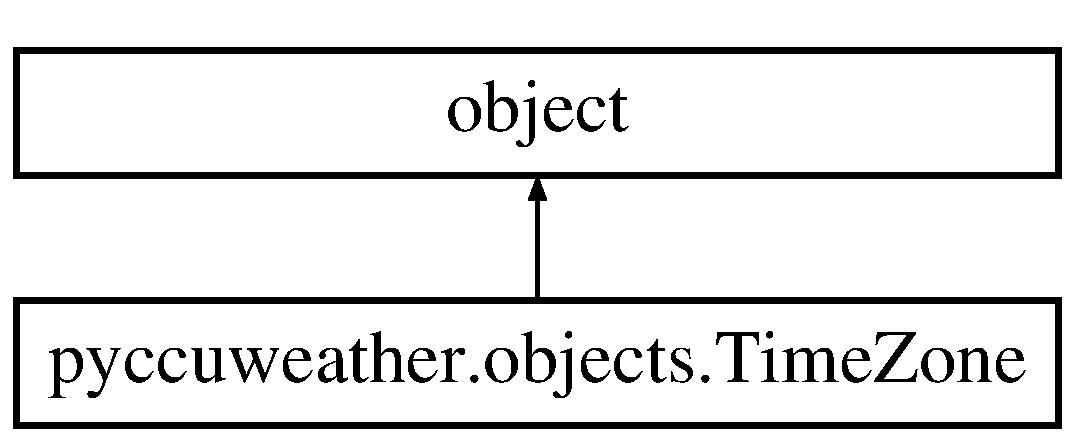
\includegraphics[height=2.000000cm]{classpyccuweather_1_1objects_1_1_time_zone}
\end{center}
\end{figure}
\subsection*{Public Member Functions}
\begin{DoxyCompactItemize}
\item 
\hypertarget{classpyccuweather_1_1objects_1_1_time_zone_a890f93b8a59b082d6f6fc7f549c3cf36}{}def {\bfseries \+\_\+\+\_\+init\+\_\+\+\_\+}\label{classpyccuweather_1_1objects_1_1_time_zone_a890f93b8a59b082d6f6fc7f549c3cf36}

\end{DoxyCompactItemize}
\subsection*{Public Attributes}
\begin{DoxyCompactItemize}
\item 
\hypertarget{classpyccuweather_1_1objects_1_1_time_zone_ad196a0ffe0d0378730db111959633c11}{}{\bfseries code}\label{classpyccuweather_1_1objects_1_1_time_zone_ad196a0ffe0d0378730db111959633c11}

\item 
\hypertarget{classpyccuweather_1_1objects_1_1_time_zone_a7626838ea0694e8b9f051eec0d289232}{}{\bfseries name}\label{classpyccuweather_1_1objects_1_1_time_zone_a7626838ea0694e8b9f051eec0d289232}

\item 
\hypertarget{classpyccuweather_1_1objects_1_1_time_zone_af8b98b5d79da281d404871417b48e66d}{}{\bfseries gmt\+\_\+offset}\label{classpyccuweather_1_1objects_1_1_time_zone_af8b98b5d79da281d404871417b48e66d}

\item 
\hypertarget{classpyccuweather_1_1objects_1_1_time_zone_a36ec251ad356cc0eee6ac5bd98ddf7c3}{}{\bfseries is\+\_\+daylight\+\_\+saving}\label{classpyccuweather_1_1objects_1_1_time_zone_a36ec251ad356cc0eee6ac5bd98ddf7c3}

\item 
\hypertarget{classpyccuweather_1_1objects_1_1_time_zone_a605ebbe8b4027d75801c96cc50c65116}{}{\bfseries next\+\_\+offset\+\_\+change}\label{classpyccuweather_1_1objects_1_1_time_zone_a605ebbe8b4027d75801c96cc50c65116}

\end{DoxyCompactItemize}


\subsection{Detailed Description}
\begin{DoxyVerb}Represents a timezone.
Timezones are explained in the Accuweather documentation at http://apidev.accuweather.com/developers/timeZones
\end{DoxyVerb}
 

The documentation for this class was generated from the following file\+:\begin{DoxyCompactItemize}
\item 
pyccuweather/objects.\+py\end{DoxyCompactItemize}

\hypertarget{classpyccuweather_1_1errors_1_1_unauthorised_error}{}\section{pyccuweather.\+errors.\+Unauthorised\+Error Class Reference}
\label{classpyccuweather_1_1errors_1_1_unauthorised_error}\index{pyccuweather.\+errors.\+Unauthorised\+Error@{pyccuweather.\+errors.\+Unauthorised\+Error}}
Inheritance diagram for pyccuweather.\+errors.\+Unauthorised\+Error\+:\begin{figure}[H]
\begin{center}
\leavevmode
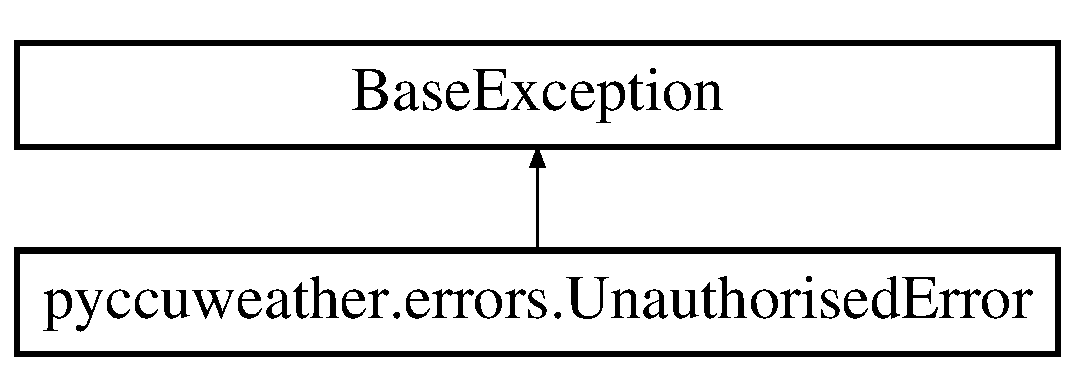
\includegraphics[height=2.000000cm]{classpyccuweather_1_1errors_1_1_unauthorised_error}
\end{center}
\end{figure}
\subsection*{Public Member Functions}
\begin{DoxyCompactItemize}
\item 
\hypertarget{classpyccuweather_1_1errors_1_1_unauthorised_error_af25f3990dca22987a786bfd85ad49404}{}def {\bfseries \+\_\+\+\_\+str\+\_\+\+\_\+} (self)\label{classpyccuweather_1_1errors_1_1_unauthorised_error_af25f3990dca22987a786bfd85ad49404}

\end{DoxyCompactItemize}


\subsection{Detailed Description}
\begin{DoxyVerb}Raised when the connection was not authorised.
\end{DoxyVerb}
 

The documentation for this class was generated from the following file\+:\begin{DoxyCompactItemize}
\item 
pyccuweather/errors.\+py\end{DoxyCompactItemize}

\hypertarget{classpyccuweather_1_1objects_1_1_wind}{}\section{pyccuweather.\+objects.\+Wind Class Reference}
\label{classpyccuweather_1_1objects_1_1_wind}\index{pyccuweather.\+objects.\+Wind@{pyccuweather.\+objects.\+Wind}}
Inheritance diagram for pyccuweather.\+objects.\+Wind\+:\begin{figure}[H]
\begin{center}
\leavevmode
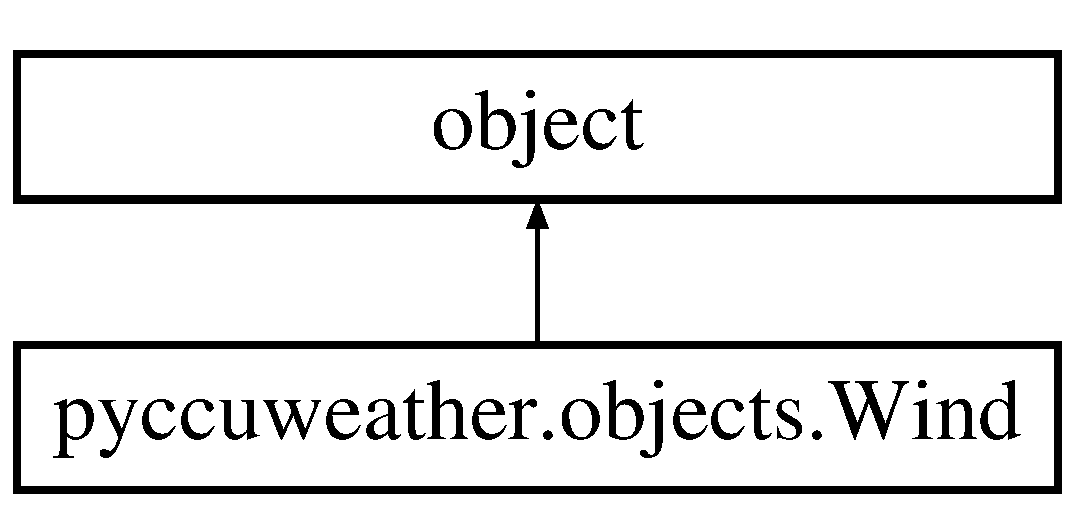
\includegraphics[height=2.000000cm]{classpyccuweather_1_1objects_1_1_wind}
\end{center}
\end{figure}
\subsection*{Public Member Functions}
\begin{DoxyCompactItemize}
\item 
\hypertarget{classpyccuweather_1_1objects_1_1_wind_a2f423b5cf45f8dd60b4b3364e5f4f3ac}{}def {\bfseries \+\_\+\+\_\+init\+\_\+\+\_\+}\label{classpyccuweather_1_1objects_1_1_wind_a2f423b5cf45f8dd60b4b3364e5f4f3ac}

\item 
\hypertarget{classpyccuweather_1_1objects_1_1_wind_ada5377451eb00b24eb0afce693e3a98f}{}def {\bfseries kmh} (self)\label{classpyccuweather_1_1objects_1_1_wind_ada5377451eb00b24eb0afce693e3a98f}

\item 
\hypertarget{classpyccuweather_1_1objects_1_1_wind_a6413e92428abdc1ebbed1e63ba16dae5}{}def {\bfseries mph} (self)\label{classpyccuweather_1_1objects_1_1_wind_a6413e92428abdc1ebbed1e63ba16dae5}

\item 
\hypertarget{classpyccuweather_1_1objects_1_1_wind_ae0582ccd76b8277739cea932778d14d0}{}def {\bfseries \+\_\+\+\_\+str\+\_\+\+\_\+} (self)\label{classpyccuweather_1_1objects_1_1_wind_ae0582ccd76b8277739cea932778d14d0}

\end{DoxyCompactItemize}
\subsection*{Public Attributes}
\begin{DoxyCompactItemize}
\item 
\hypertarget{classpyccuweather_1_1objects_1_1_wind_aa3b836245385c31cbd94a9c5be8a4cfd}{}{\bfseries speed}\label{classpyccuweather_1_1objects_1_1_wind_aa3b836245385c31cbd94a9c5be8a4cfd}

\item 
\hypertarget{classpyccuweather_1_1objects_1_1_wind_aaeb472949e84e3dea1f1267c490ff49f}{}{\bfseries units}\label{classpyccuweather_1_1objects_1_1_wind_aaeb472949e84e3dea1f1267c490ff49f}

\item 
\hypertarget{classpyccuweather_1_1objects_1_1_wind_a751506b75edac12a8bcc7965083f5aec}{}{\bfseries hdg}\label{classpyccuweather_1_1objects_1_1_wind_a751506b75edac12a8bcc7965083f5aec}

\end{DoxyCompactItemize}


The documentation for this class was generated from the following file\+:\begin{DoxyCompactItemize}
\item 
pyccuweather/objects.\+py\end{DoxyCompactItemize}

%--- End generated contents ---

% Index
\backmatter
\newpage
\phantomsection
\clearemptydoublepage
\addcontentsline{toc}{chapter}{Index}
\printindex

\end{document}
